\begin{savequote}[8cm]
  ``I've always believed that if you put in the work, the results will come.''
  \qauthor{Michael Jordan}
\end{savequote}
\makeatletter
\chapter{Results}

\section{Results}

\section{Qualitative Results}

\section{Quantitative Results}

\subsection{Pose Estimation Results}

These experiments measured registration error for the data sets mentioned in the test data section. As mentioned, different camera movements and scene types are used. Different camera movements such as translation, rotation and zoom were used. The different scenes used include: in-door, out-door, low-textured areas, large object frames areas and areas which include texture confusion. \\


\begin{figure*}[t]
\centering
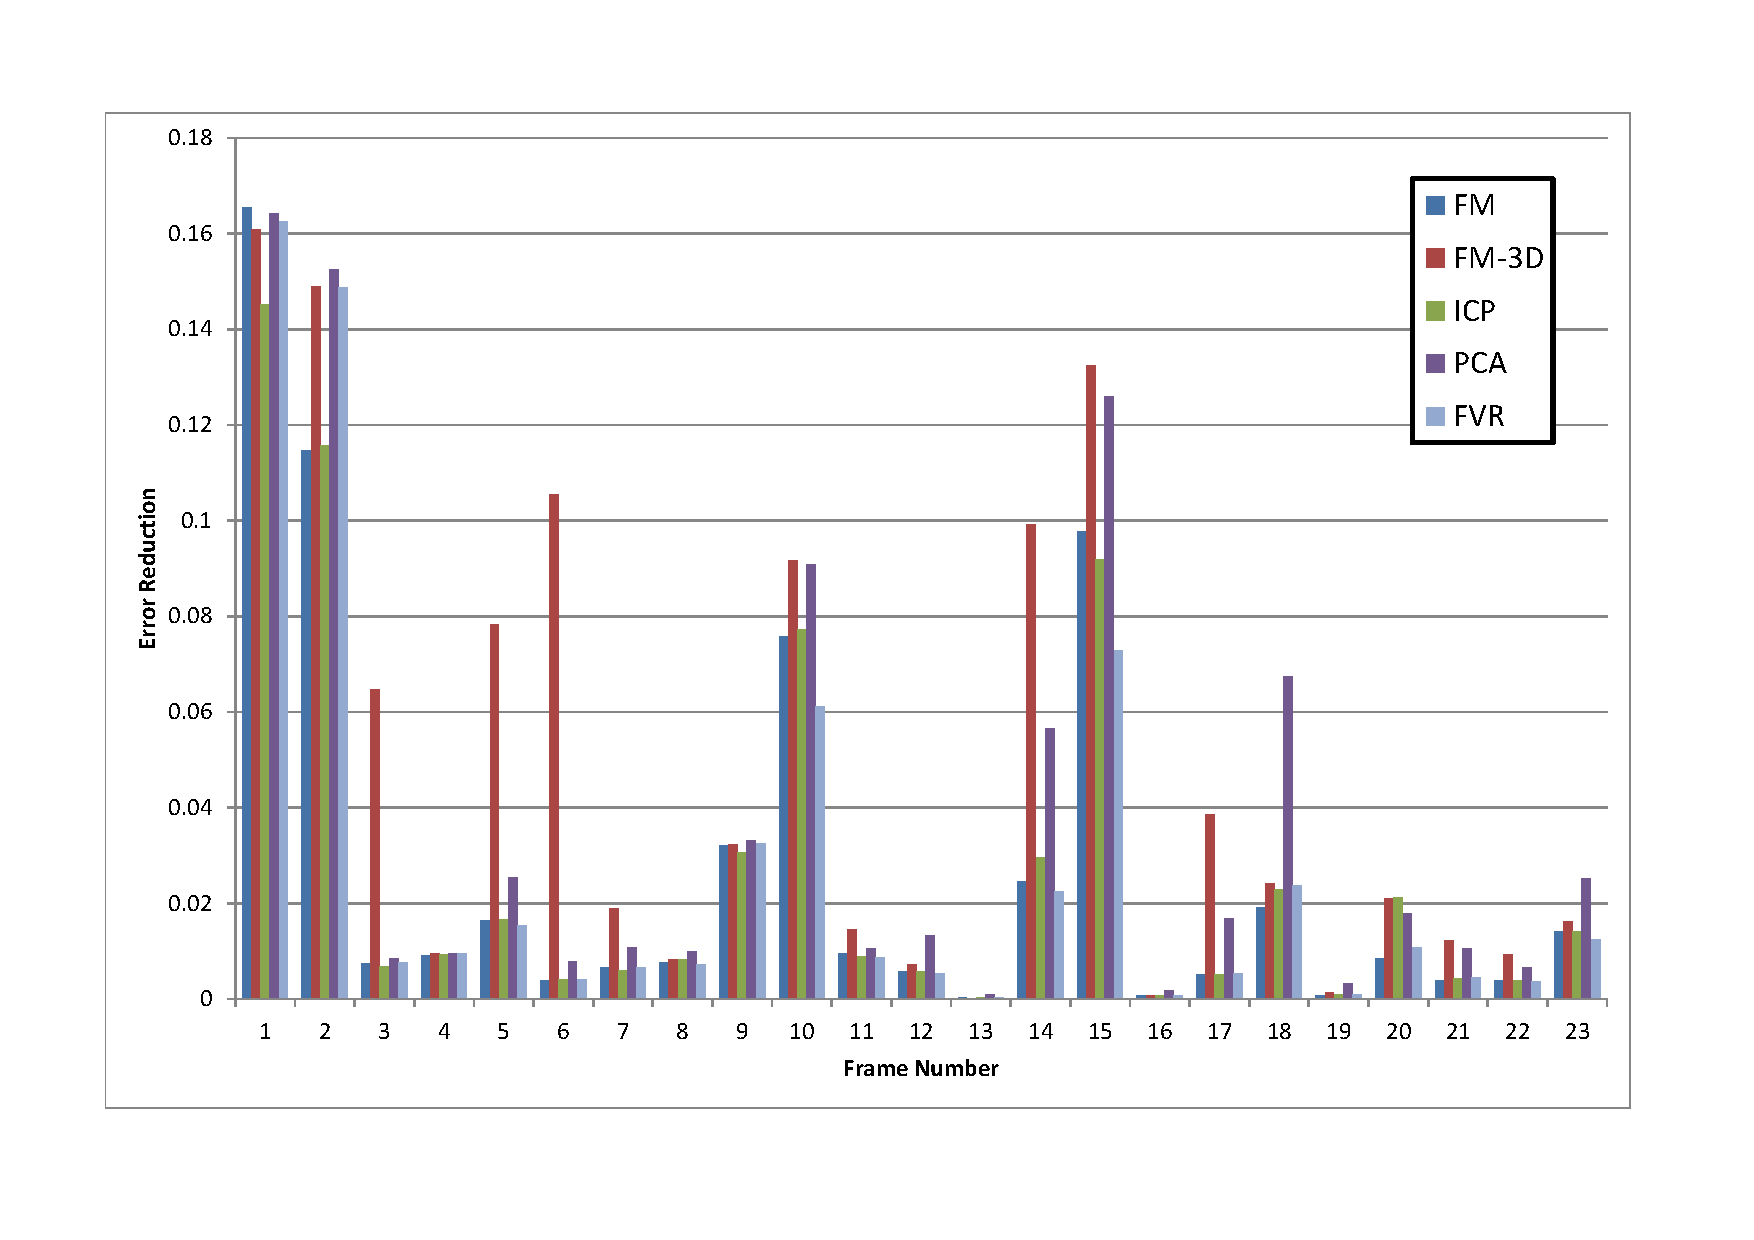
\includegraphics[width=6.0in]{images/results/Apartment_Texture_Rotate}
\caption{Registration Error for the Apartment Y-Axis Rotation Data Set}
\label{fig:PET0}
\end{figure*}

The first experiment was performed with the textured apartment data-set \ref{fig:PET0}. In each of these graphs, the x-axis represents the frame number (in which the previous frame was matched to) and the y-axis represents the registration error in Hausdorff distance relative to performing zero registration. For identical point-clouds, a Hausdorff error above 1 would mean a failure to register in any way, whilst a 0 would mean a complete registration. Since frames do not overlap, it would be improbably to get 0, and a registration error of 1 or above may still be considered good, especially if there was not much overlap in the first place. \\


\begin{figure*}[t]
\centering
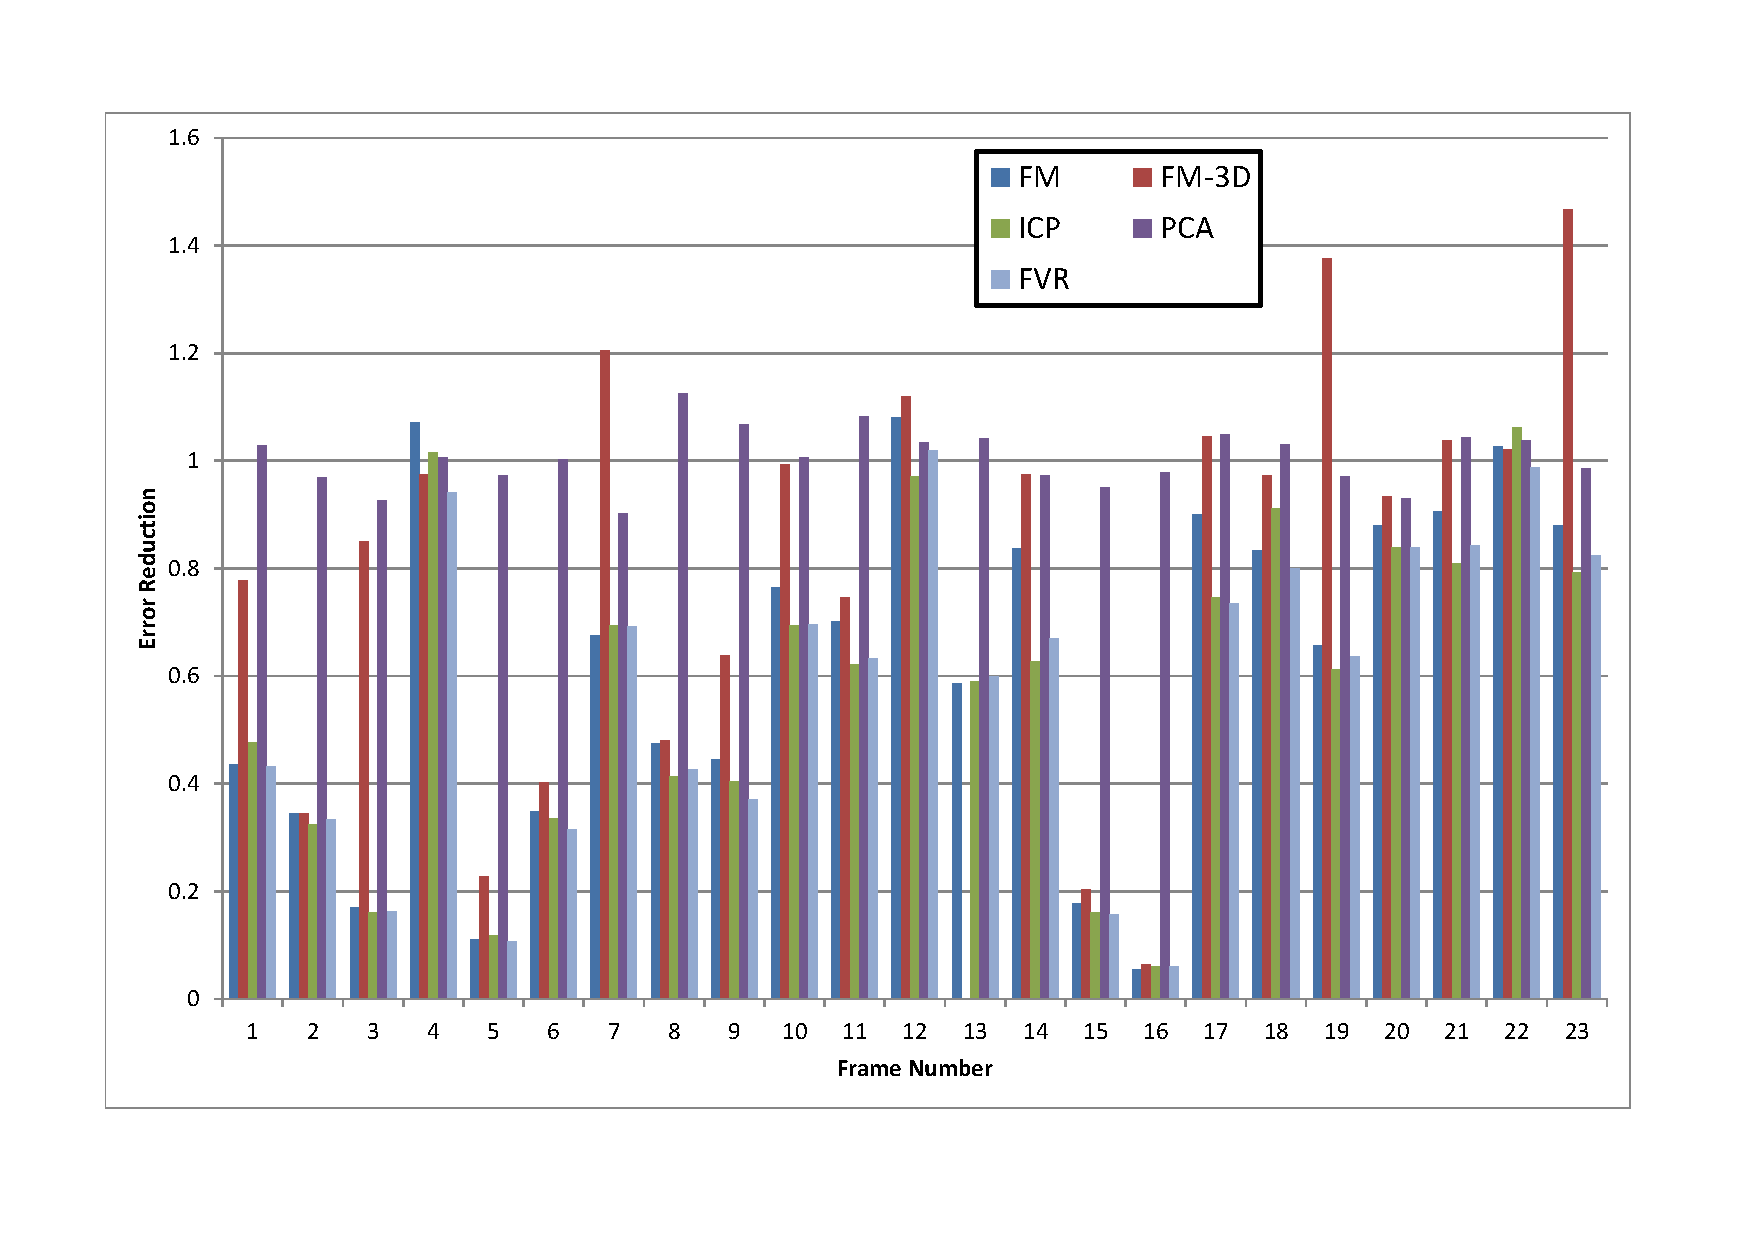
\includegraphics[width=6.0in]{images/results/Apartment_Texture_Rotate_XAxis}
\caption{Registration Error for the Apartment X/Y-Axis Rotation Data Set}
\label{fig:PET1}
\end{figure*}

In figure \ref{fig:PET0}, feature-matching, 3D-feature-matching, ICP, PCA and Fourier Volume Registration (FVR) were tested. In the first frame, FVR only outperformed feature-matching and PCA. In a few of the frames, the 3D feature matching and the PCA methods performed poorly relative to the reset, on other frames they were on par with others. In some frames FVR outperformed the others, this occurred on 13 out of the 23 frames tested (about 60\%). This was not completely expected as for this scene, where much texture is present, feature matching should have dominated. The frames were not highly separated so ICP should have gotten a better result too. Although ICP could be said to be very consistent.

\begin{figure*}[t]
\centering
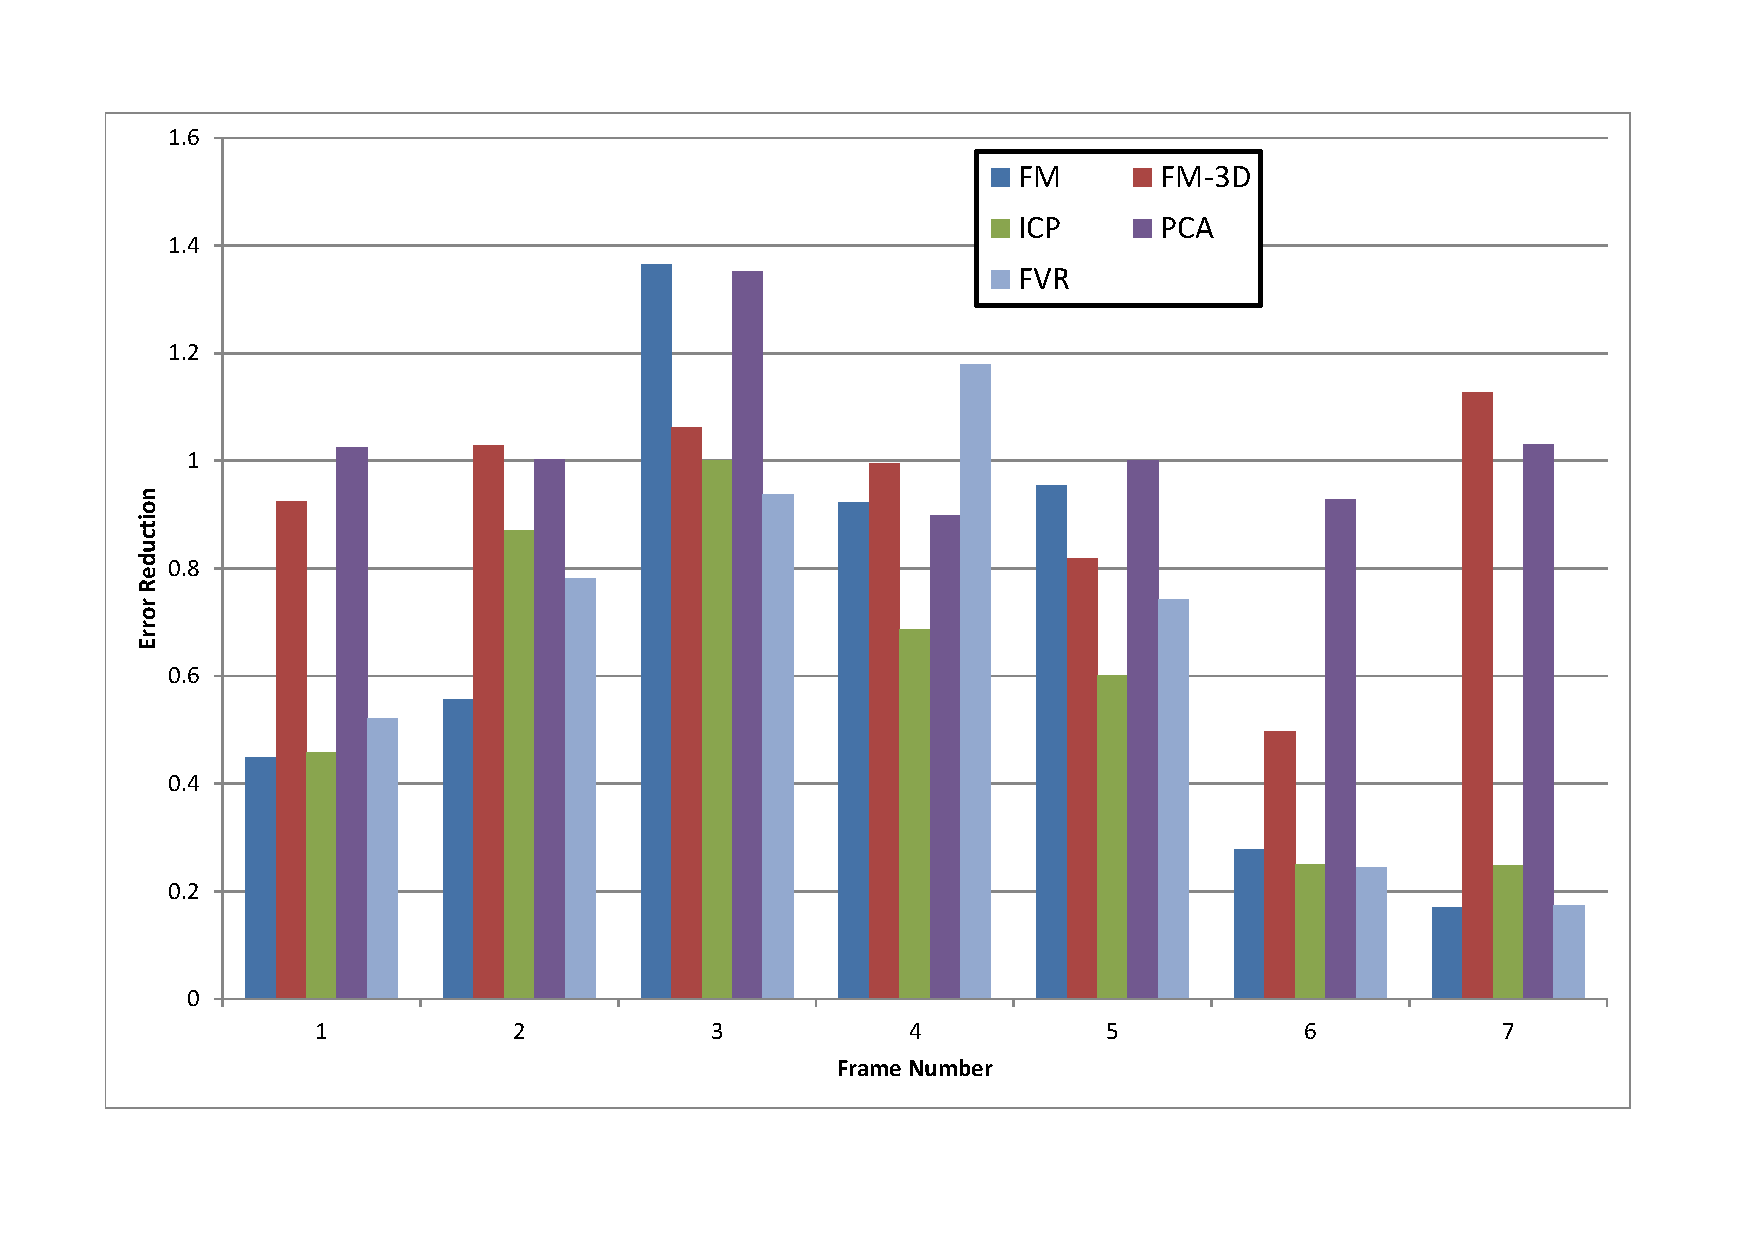
\includegraphics[width=6.0in]{images/results/Boxes_Texture_Rotate}
\caption{Registration Error for the Boxes Y-Axis Rotation Data Set}
\label{fig:PET2}
\end{figure*}

Figure \ref{fig:PET1} shows registration errors for the same scene, the apartment, this time the camera is moved about the x-axis predominantly, again it contains lots of texture. In a about 60\% of the frames, FVR either outperforms or matches the best performing algorithm. Here, ICP and 2D-feature matching are also very competitive, with 3D-feature-matching and PCA failing. In the case of PCA, when there is not enough overlap PCA fails to compute the principal components well. When FVR uses PCA, it only uses the primary axis, and can iteratively refine the alignment in a second stage.

\begin{figure*}[t]
\centering
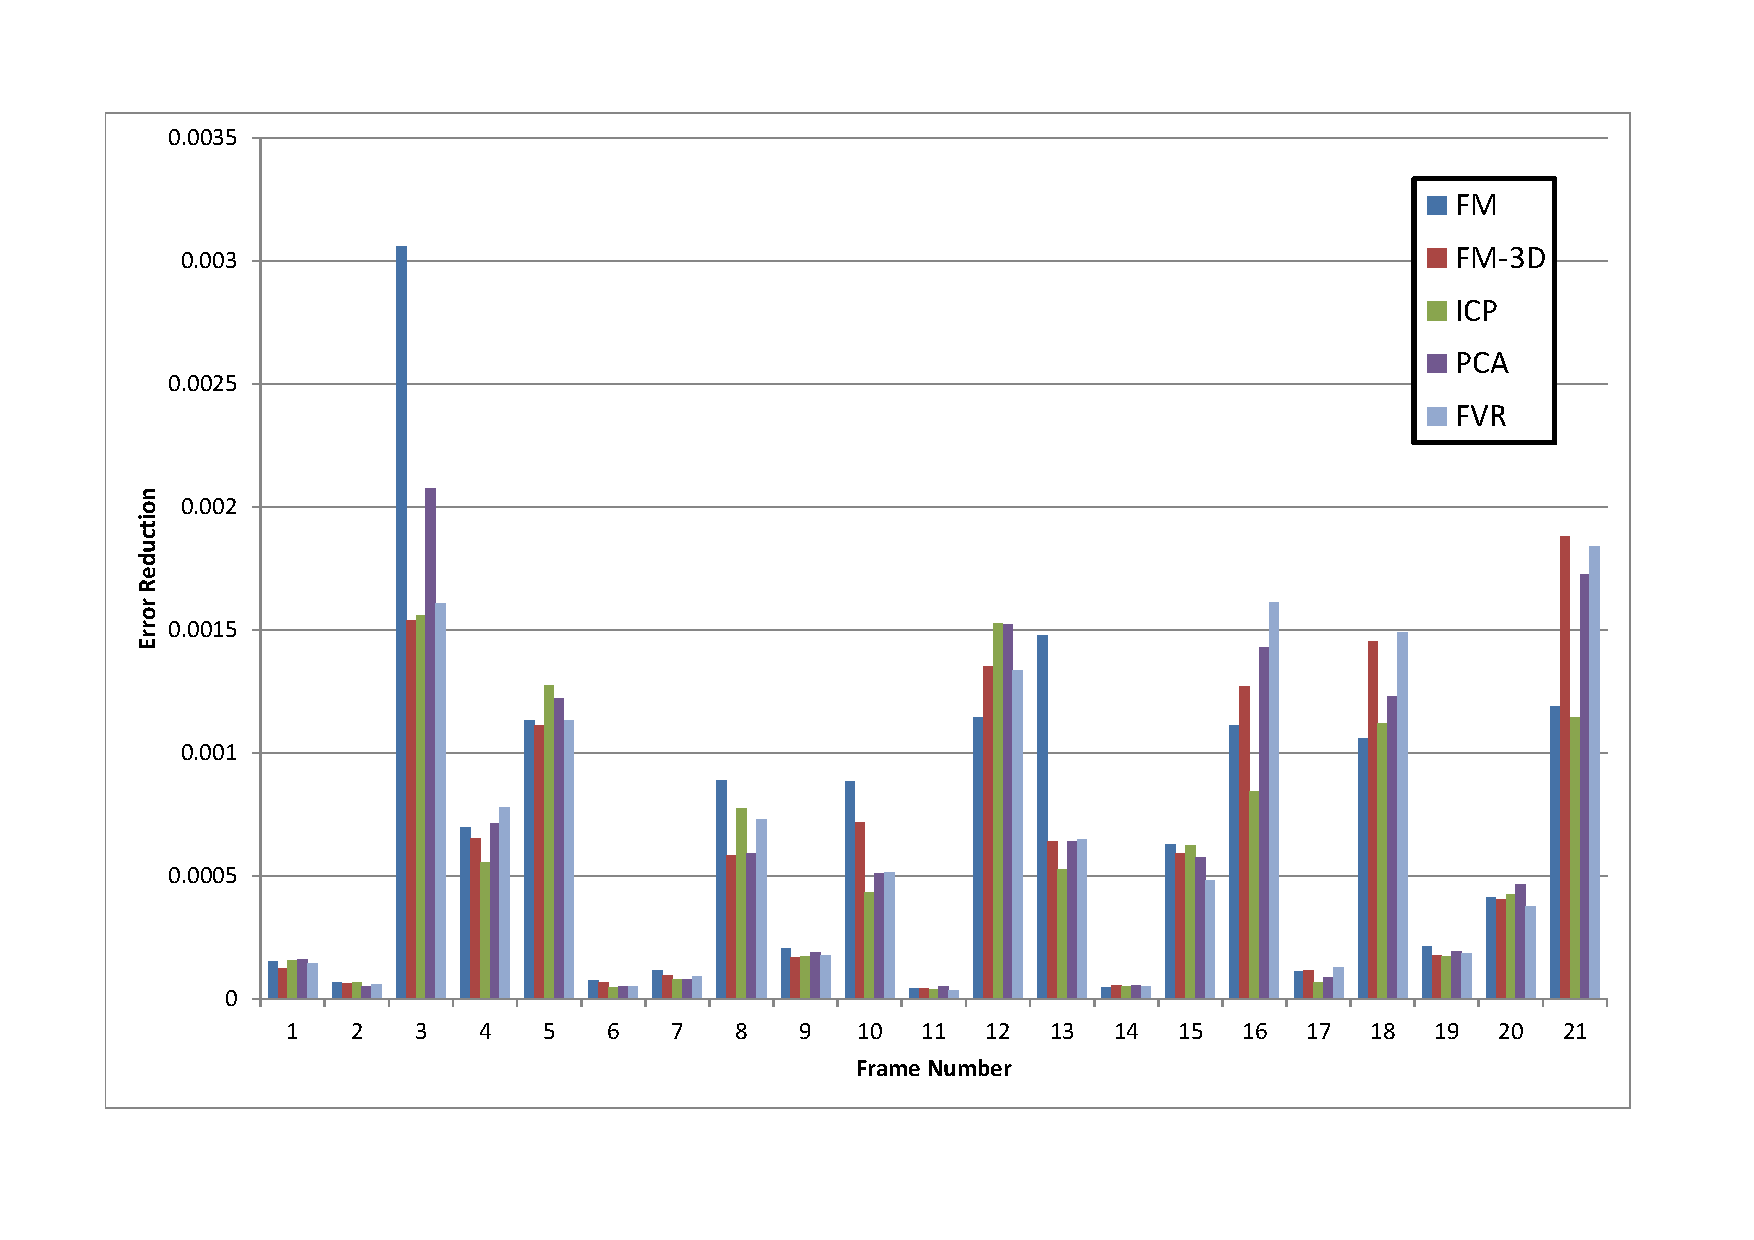
\includegraphics[width=6.0in]{images/results/Boxes_Texture_ZoomOut}
\caption{Registration Error for the Boxes Zoom Data Set}
\label{fig:PET3}
\end{figure*}

In figure \ref{fig:PET2} 7 registration errors are shown in a graph. In 4 out of the 7 frames, FVR outperformed the other algorithms. Note in frame 3, both PCA and feature-matching failed, despite texture being present in the scene. In frames 4 and 5, ICP outperformed the others by a successful margin. 

\begin{figure*}[t]
\centering
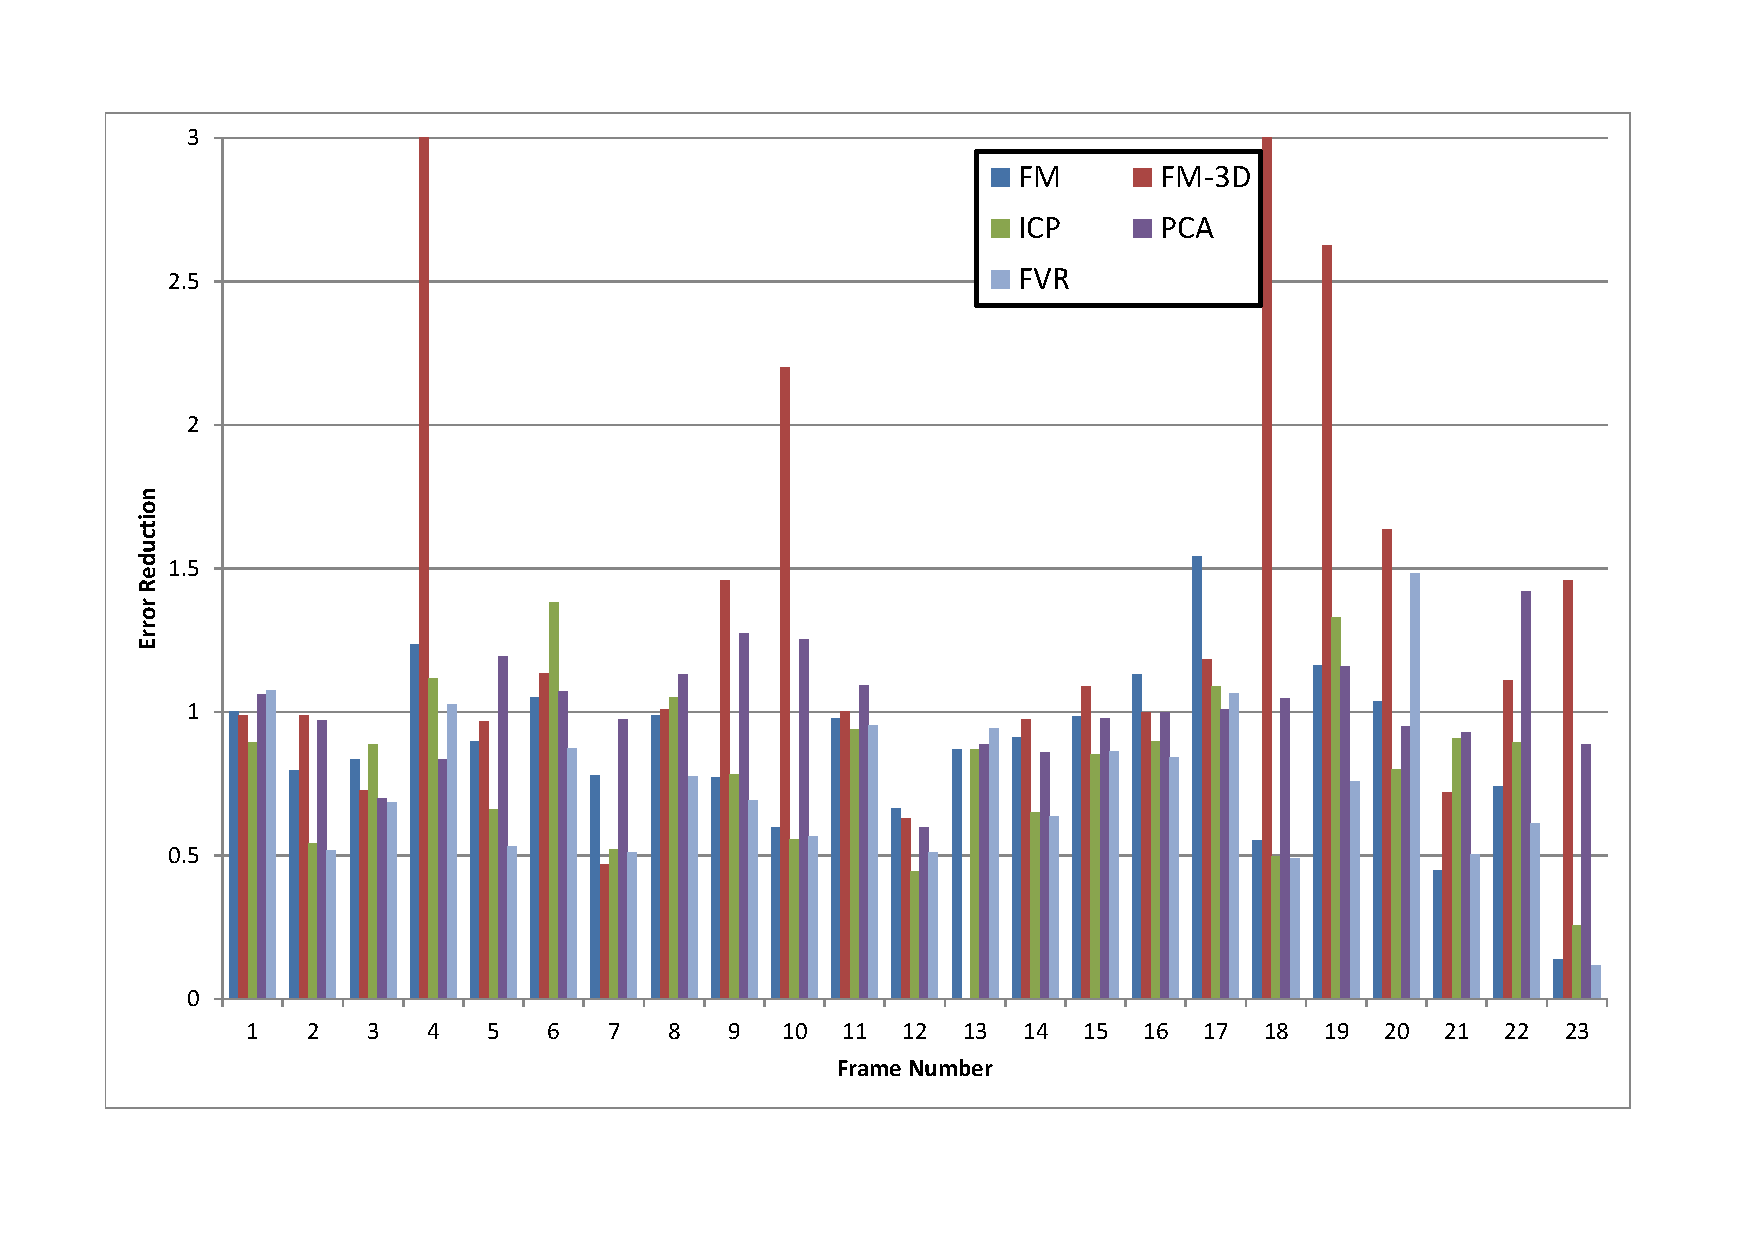
\includegraphics[width=6.0in]{images/results/Desk_Texture_Translation}
\caption{Registration Error for the Desk Translation Data Set}
\label{fig:PET4}
\end{figure*}

Experiment results for the boxes scene where the camera was moved forward, effectively zooming in on the boxes, are shown in figure \ref{fig:PET3}. Here, only 10 out of the 21 (~47\%) of the frames had a registration error lowest or equal for FVR. In a rare case, frame 16 observed a worst performance by FVR. In frame 3, 2D-feature-matching performed the worst, and towards the last few frames PCA and 3D-feature-matching performed worst.

\begin{figure*}[t]
\centering
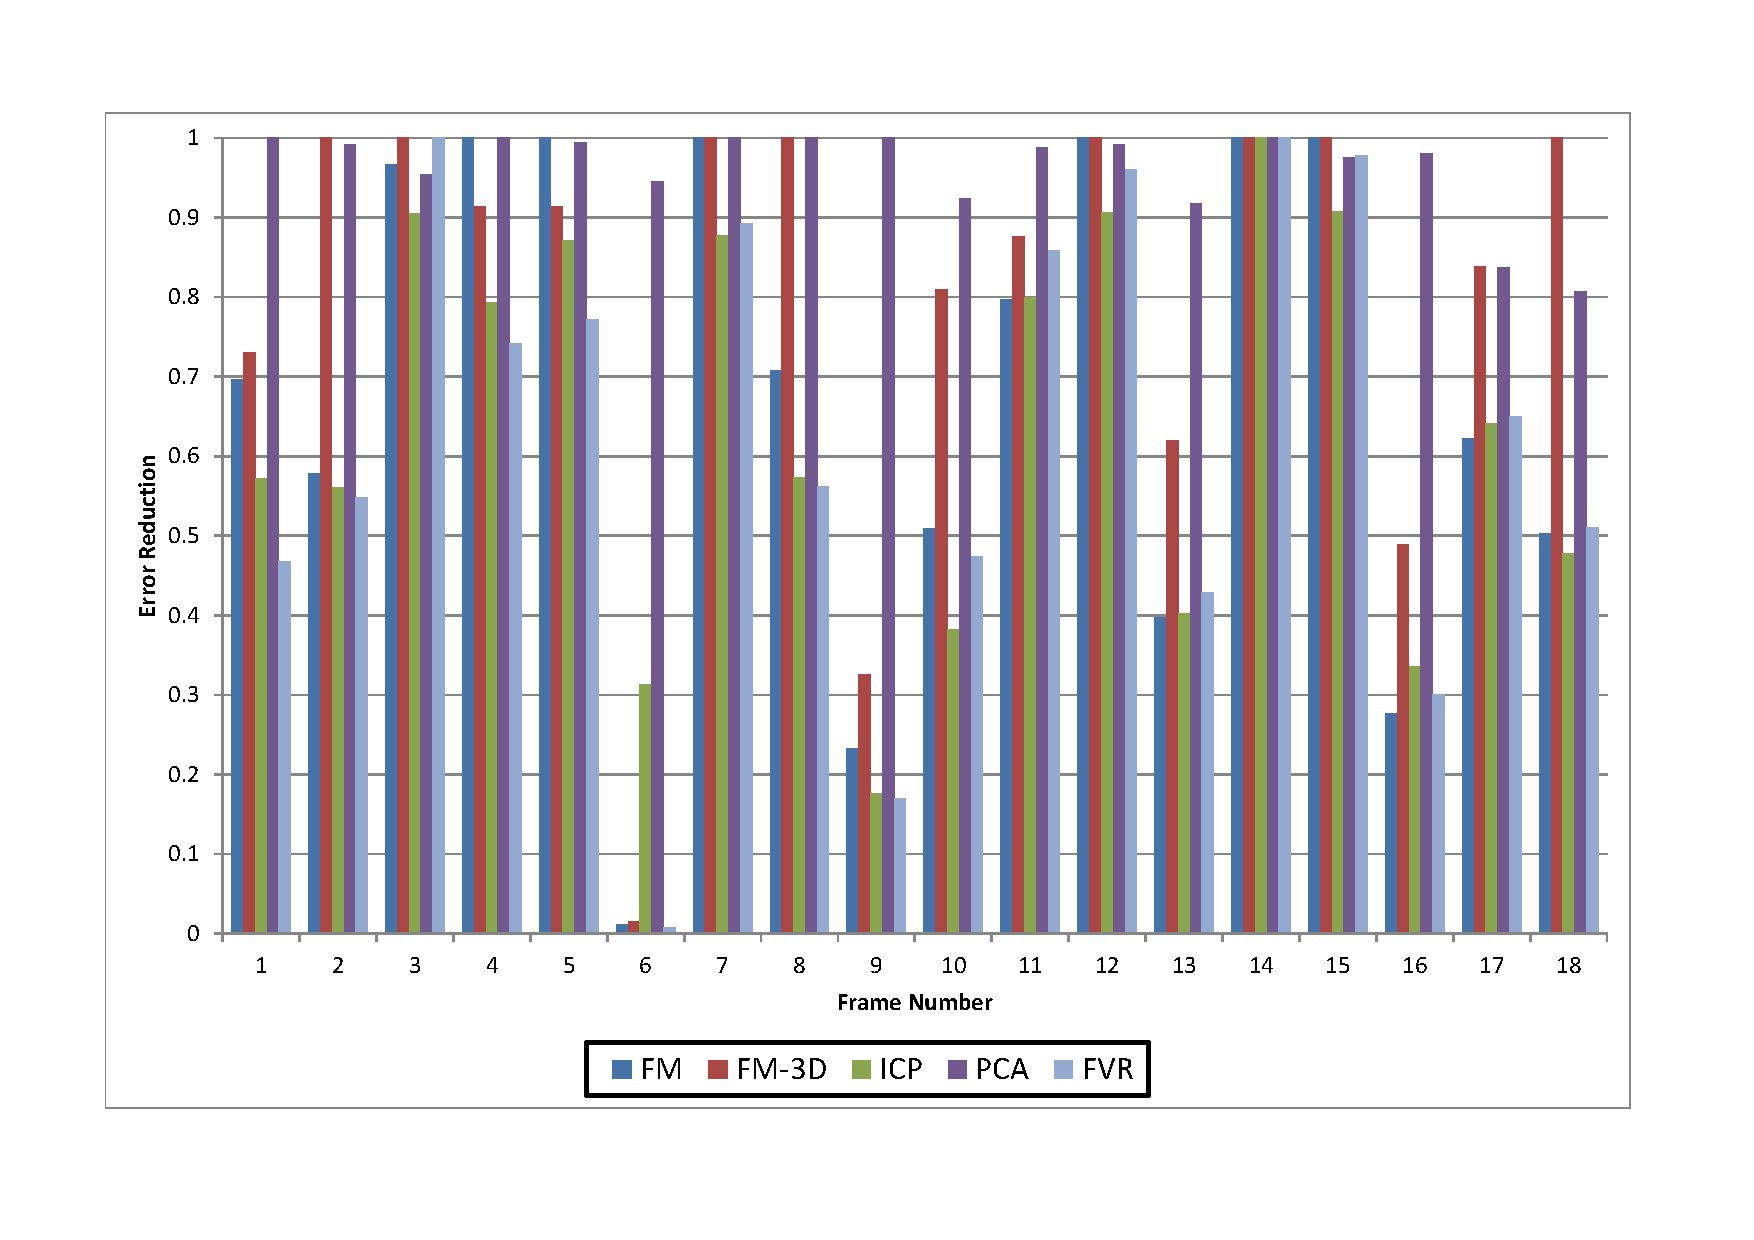
\includegraphics[width=6.0in]{images/results/IndoorSpace_texture_confusion_translation}
\caption{Registration Error for the Texture Confusion Indoor-Space Translation Data Set}
\label{fig:PET5}
\end{figure*}

In ~52\% of the frames of the desk translation data-set in figure \ref{fig:PET4}, the FVR method outperformed others relative to just ~26\% for ICP, ~9\% for 2D-feature-matching and PCA and ~4\% for 3D-feature-matching. This data-set tested for the pose-estimation procedure's ability to align a moving camera along a path. 3D feature matching was a notable poor performer here, ICP and FVR seemed to be strongest. 


\begin{figure*}[t]
\centering
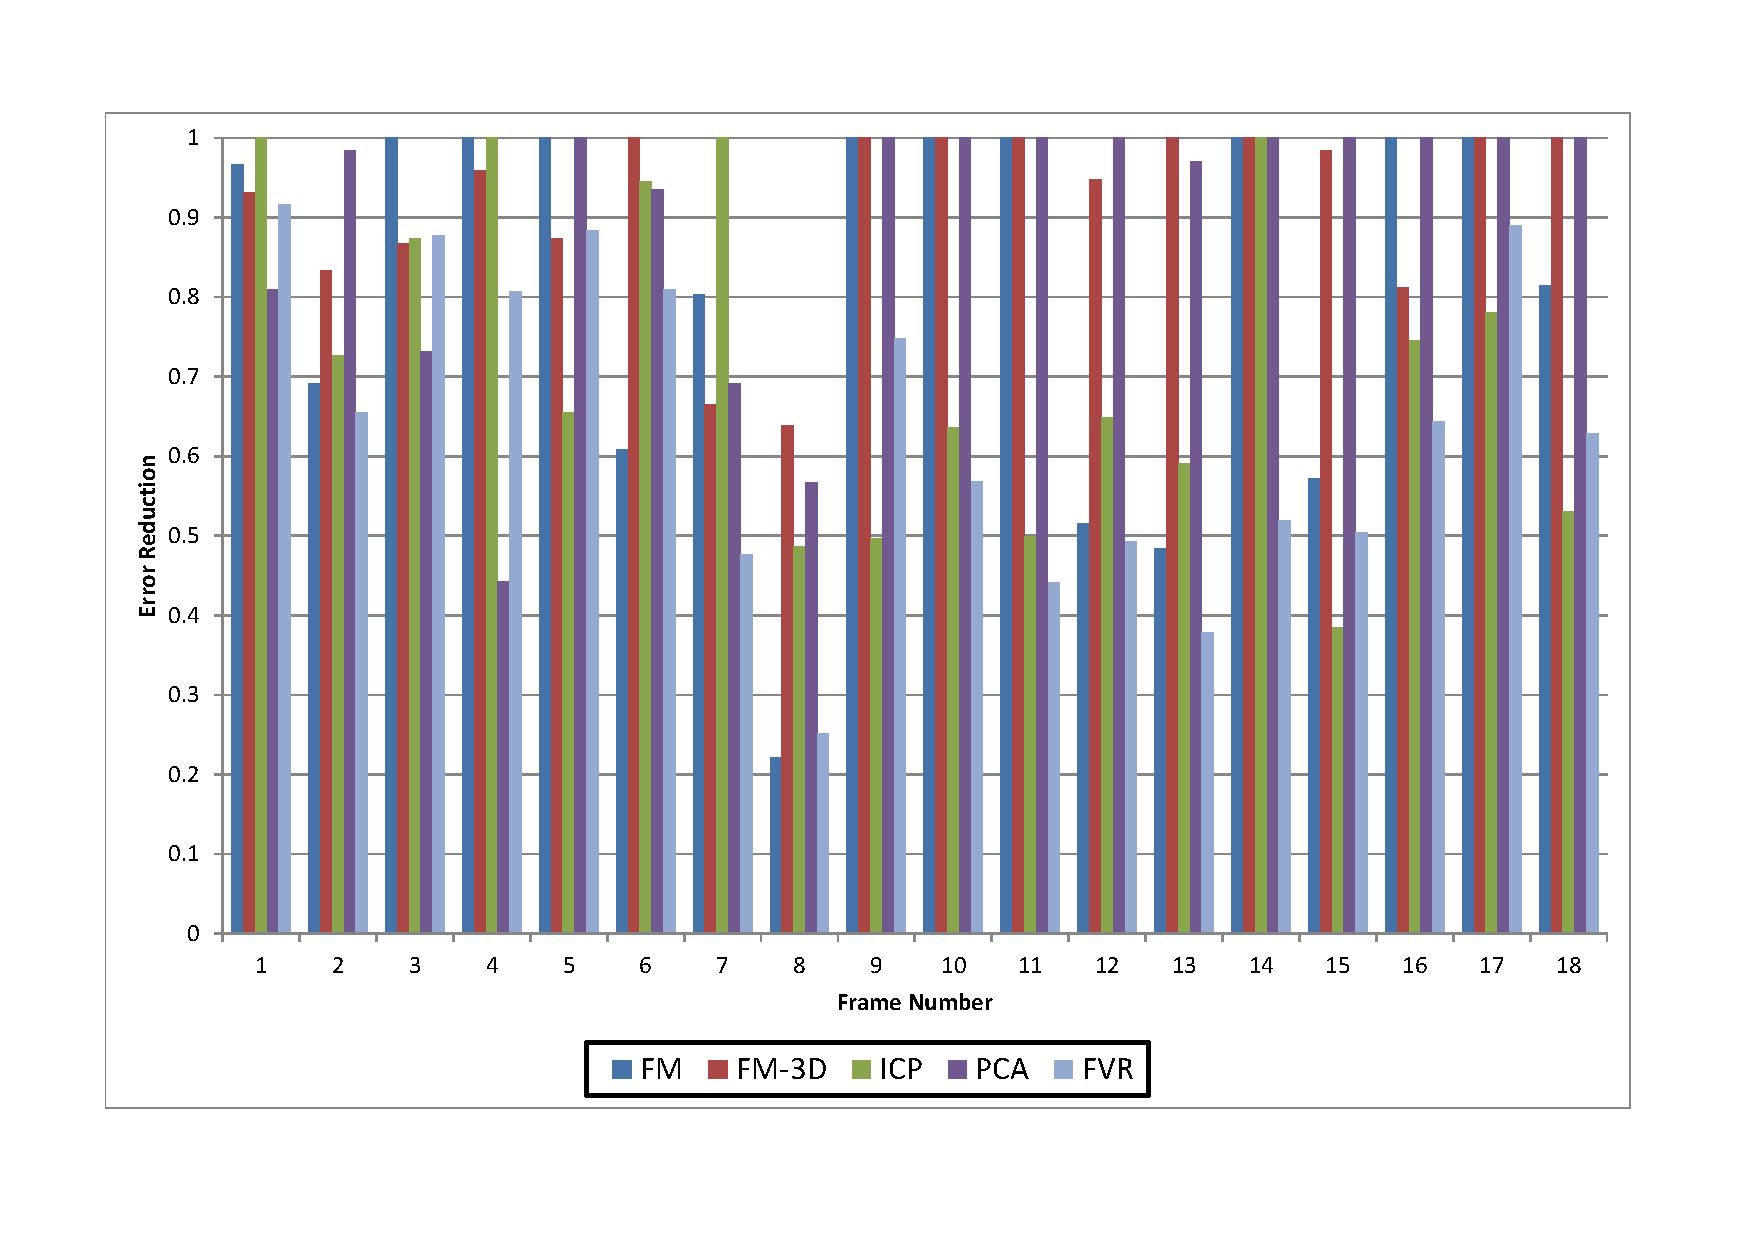
\includegraphics[width=6.0in]{images/results/Kitchen_LittleTexture_Pan}
\caption{Registration Error for the Low-Texture Kitchen Translation Data Set}
\label{fig:PET6}
\end{figure*}

An important data-set tested is the Indoor-Space with texture confusion (figure \ref{fig:PET5}). Here, a small scene was observed, where texture-confusion was present, this makes registration more difficult for all algorithms most notably the feature matching methods. We suspected that ICP, PCA, and FVR would perform best here. Here, around 39\% of the time, FVR performed best. Compared to the best feature-matching method (2D) with ~22\% of performances being the best. Interestingly PCA performed much worse compared with 2D-feature-matching. ICP outperformed others around 33\% of the time, similar to FVR's position but not quite as good. 

Results for the low-textured Kitchen data-set were collected and shown in figure \ref{fig:PET6}. Again around 44\% of the frames had best results given by FVR. Compared with the next best algorithm ICP at ~27\%. In this case, this is expected as the feature-matching methods should perform worse in a low-textured scene. PCA was next best having the best registration ~22\% of the time.

\begin{figure*}[t]
\centering
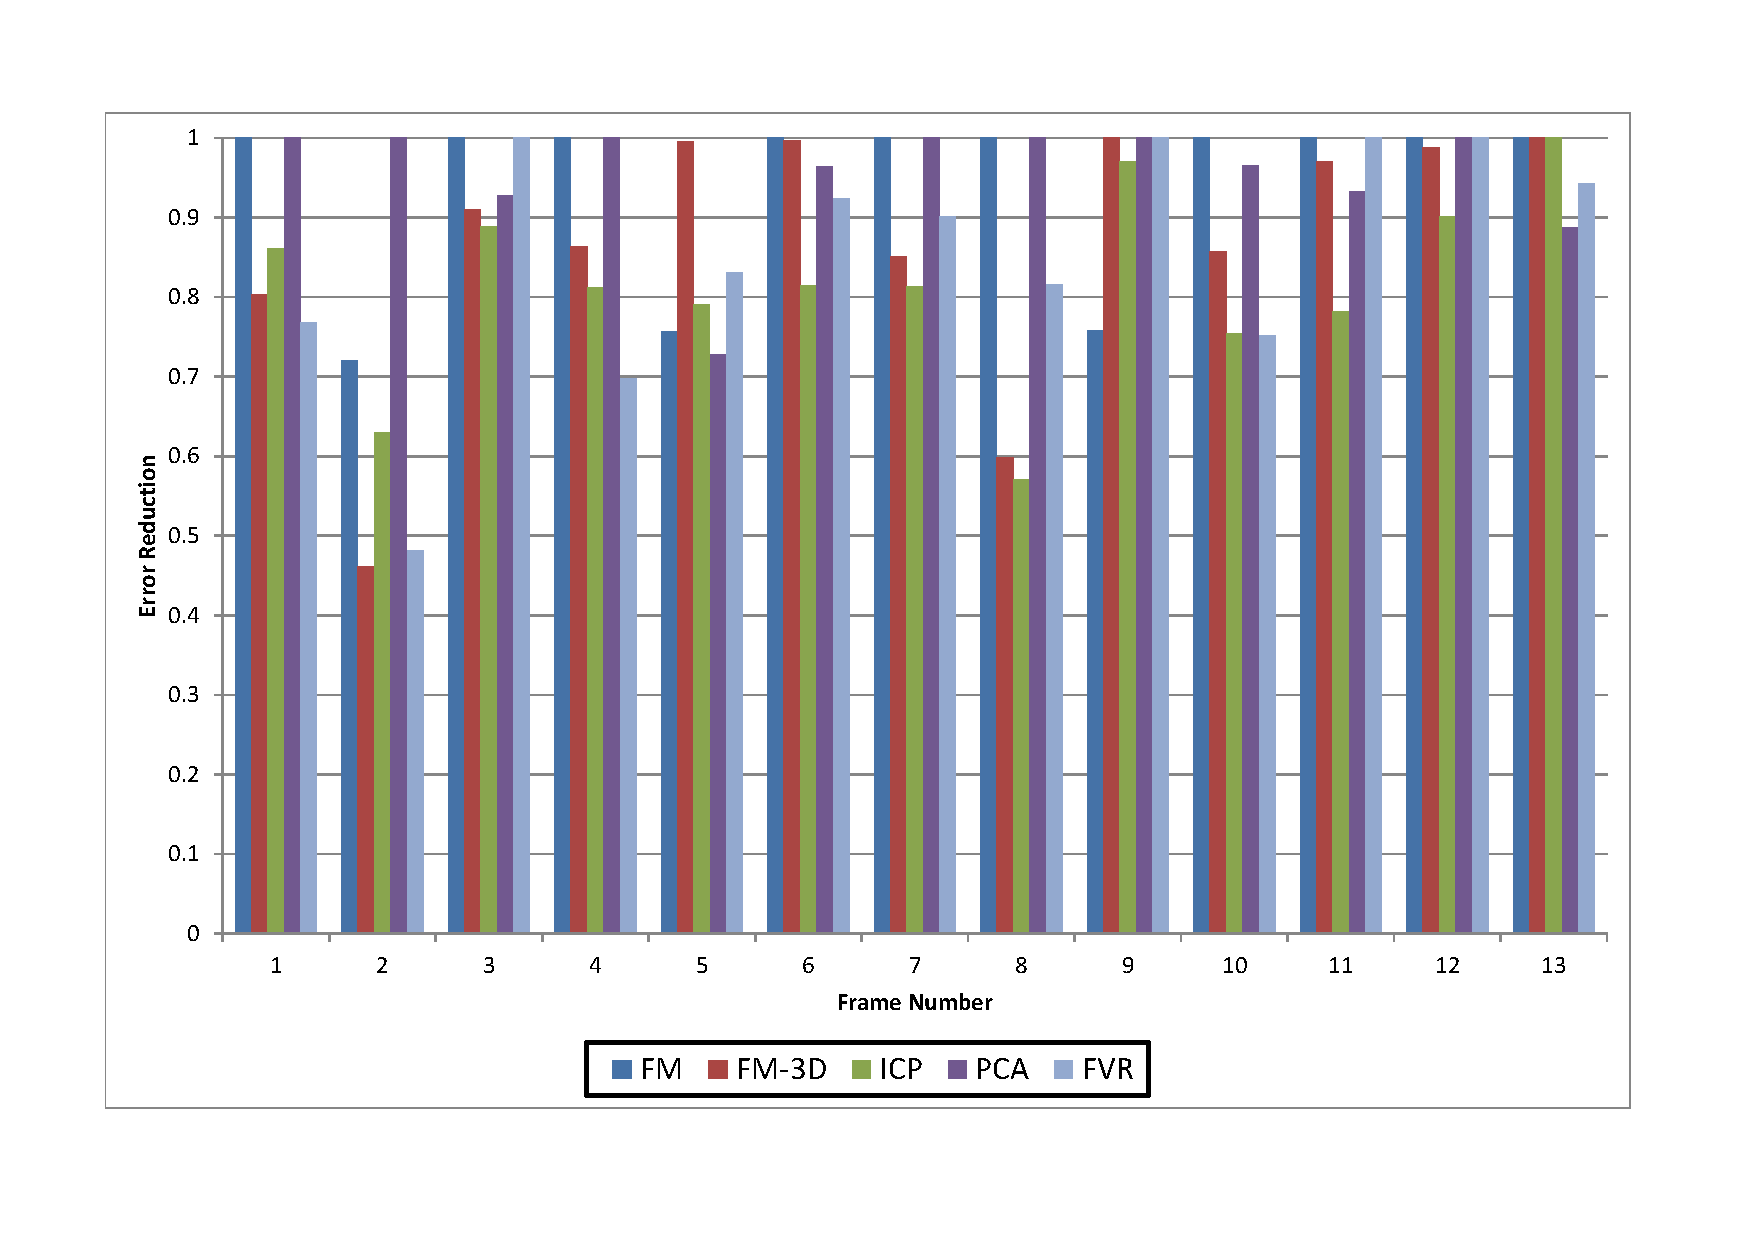
\includegraphics[width=6.0in]{images/results/Kitchen_Little_Texture_Zoom}
\caption{Registration Error for the Low-Texture Kitchen Zoom Data Set}
\label{fig:PET7}
\end{figure*}

Another test for the low-textured Kitchen scene was also performed, this time by moving the camera forward and backwards, zooming in on the scene. In this test, FVR only outperformed the other methods in 3 out of the 13 frames. ICP outperformed FVR on this data-set, as 6 out of the 5 frames had best results given by ICP. It could also be said that ICP was a little more consistent. Interestingly 3D-feature-matching outperformed the 2D counterpart.

\begin{figure*}[t]
\centering
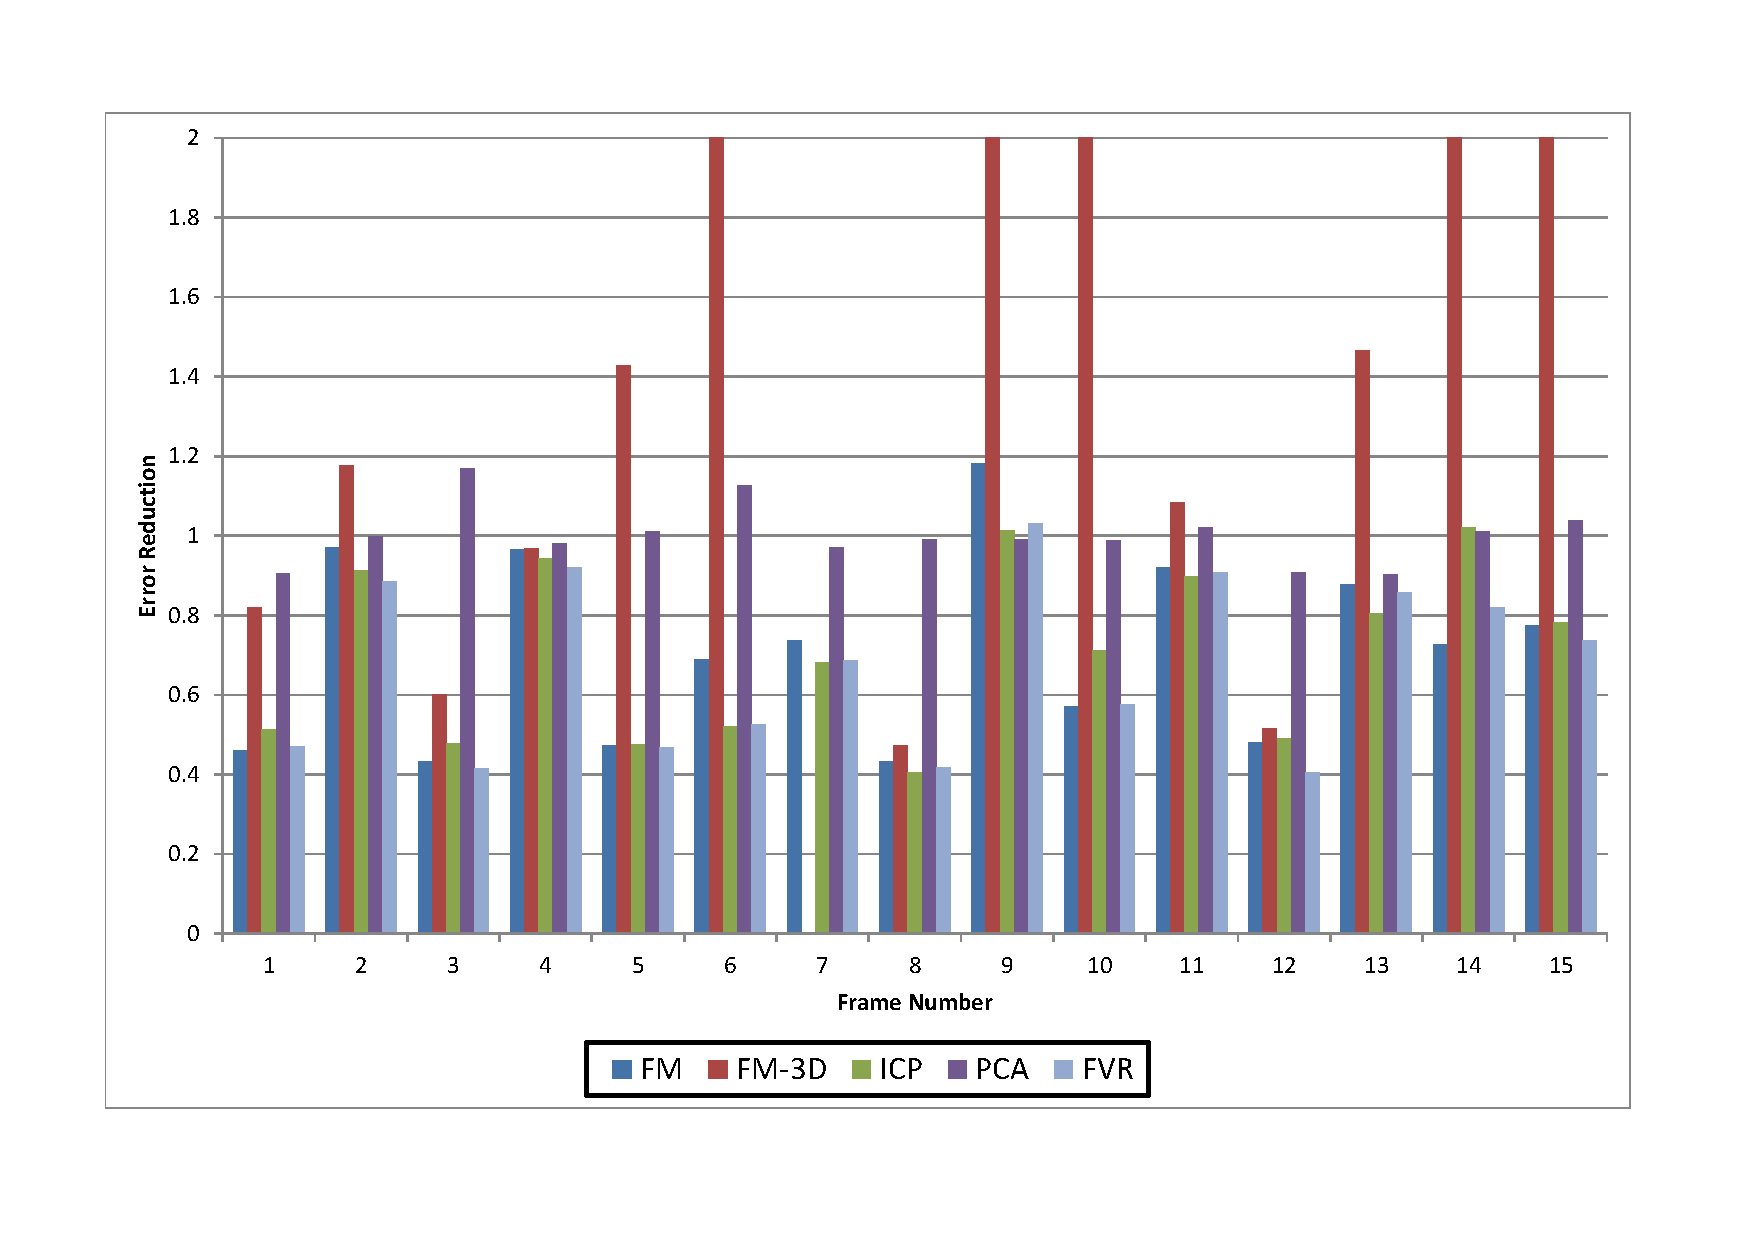
\includegraphics[width=6.0in]{images/results/Office_TexturedItems_Translation}
\caption{Registration Error for the Office Translation Data Set}
\label{fig:PET8}
\end{figure*}

In the results for the Textured Office set (figure \ref{fig:PET8}), FVR matched or beat the other algorithms 80\% of the time. 2D-feature matching also performed well but did not manage to best FVR most of the time. This results shows that, to our surprise, FVR not only works well compared to other algorithms in scenes with little or no texture or in scenes where feature confusion is high, but also in high texture scenes where feature-matching should have an advantage.


\begin{figure*}[t]
\centering
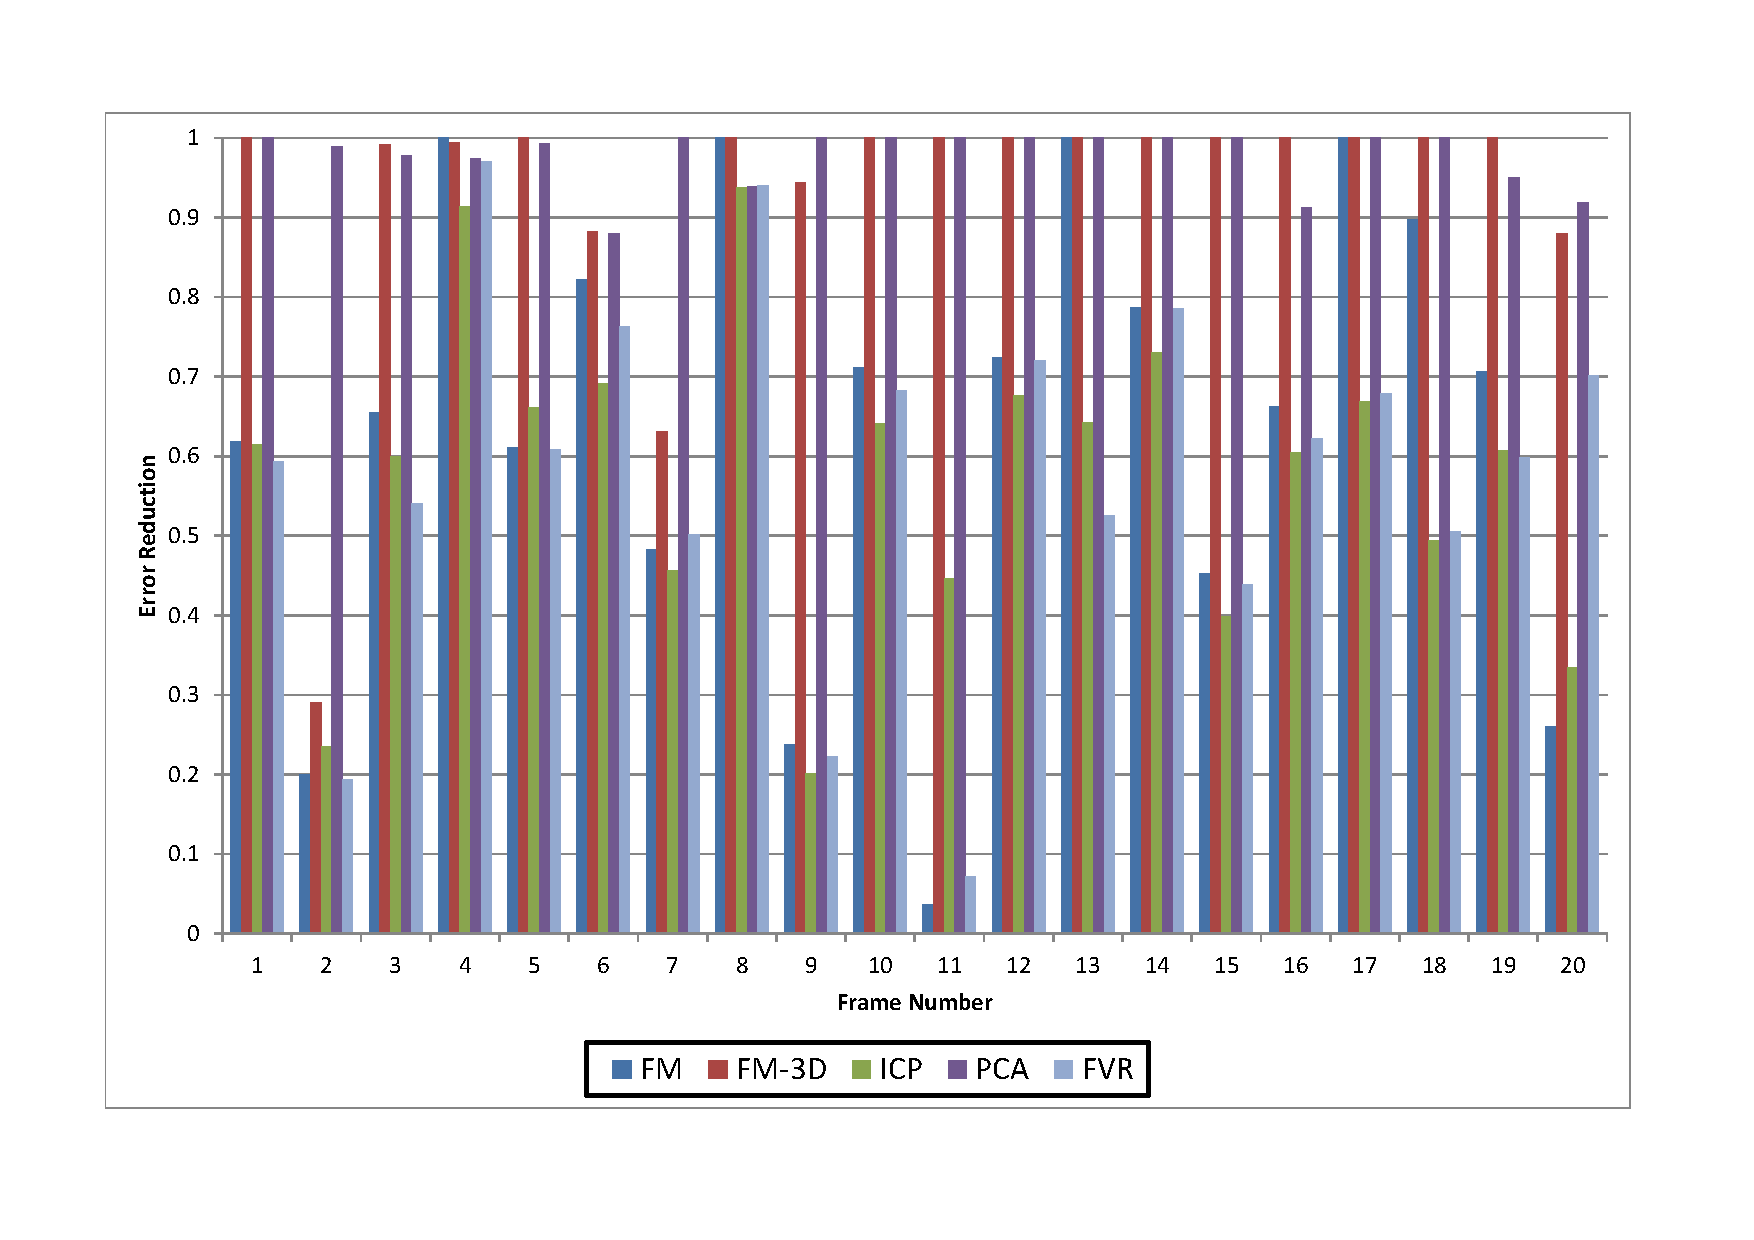
\includegraphics[width=6.0in]{images/results/Office_Texture_blind_spot_rotation}
\caption{Registration Error for the Office Centered Object Rotation Data Set}
\label{fig:PET9}
\end{figure*}

Figure \ref{fig:PET9} shows results for the centred object rotation scene. Here, a large divider was placed in the middle of two desks. The idea was to create an environment where the large divider could throw off the effects of PCA and FVR and give an advantage to the feature matching approaches and ICP. Interestingly, around 35\% of the time, FVR had the best result. 2D-feature-matching outperformed the 3D counterpart but only got the best result 10\% of the time. ICP on the other hand got the best result for around 55\% of the frames. It is suspected that ICP is able to use the large divider as an anchor which would make it more robust to non-overlapped data.

\begin{figure*}[t]
\centering
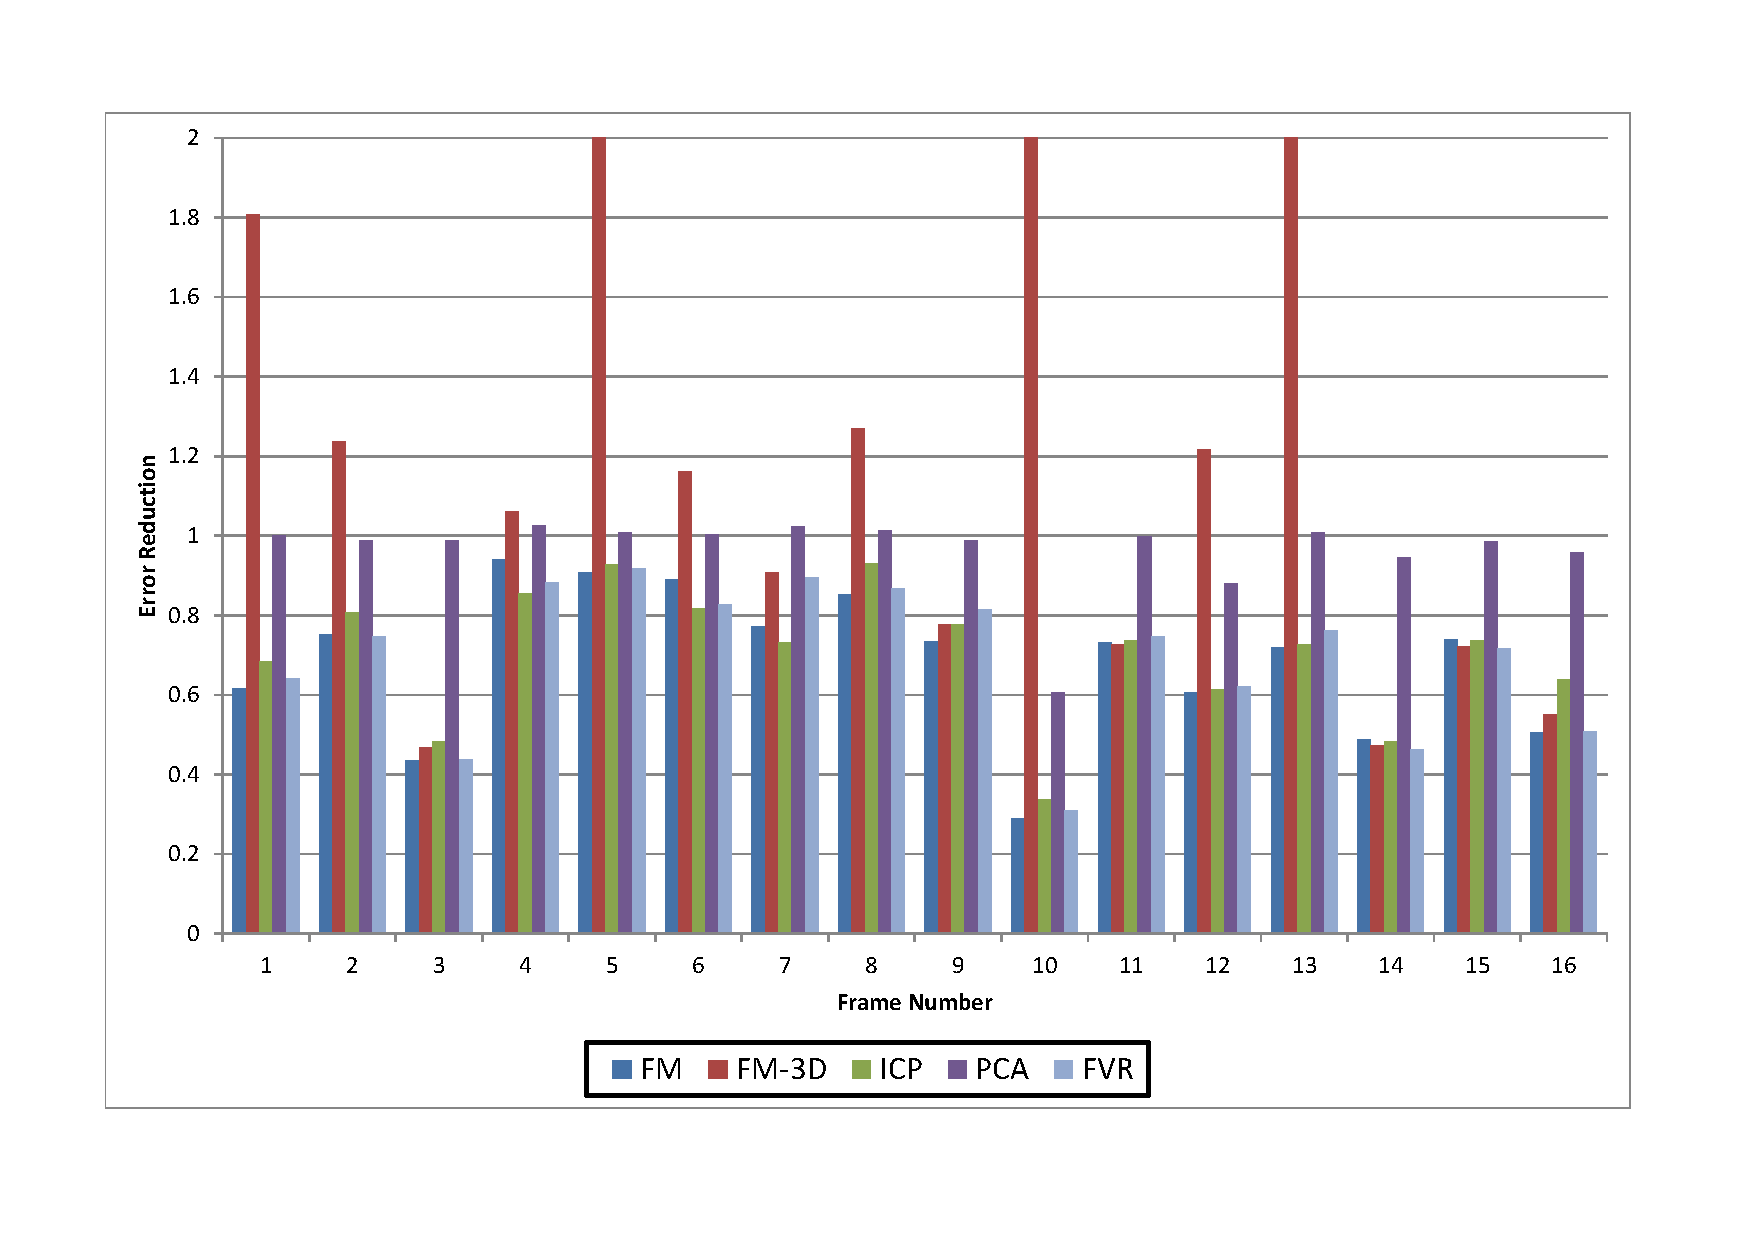
\includegraphics[width=6.0in]{images/results/Office_Texture_Rotate_XAxis}
\caption{Registration Error for the Office X/Y-Axis Rotation Data Set}
\label{fig:PET10}
\end{figure*}

Another experiment where the scene was filmed with the camera rotated predominantly about the x-axis is shown in figure \ref{fig:PET10}, this time 2D-feature-matching, ICP and FVR all performed similarly, with only PCA and 3D-feature-matching failing to get good registrations. 

\begin{figure*}[t]
\centering
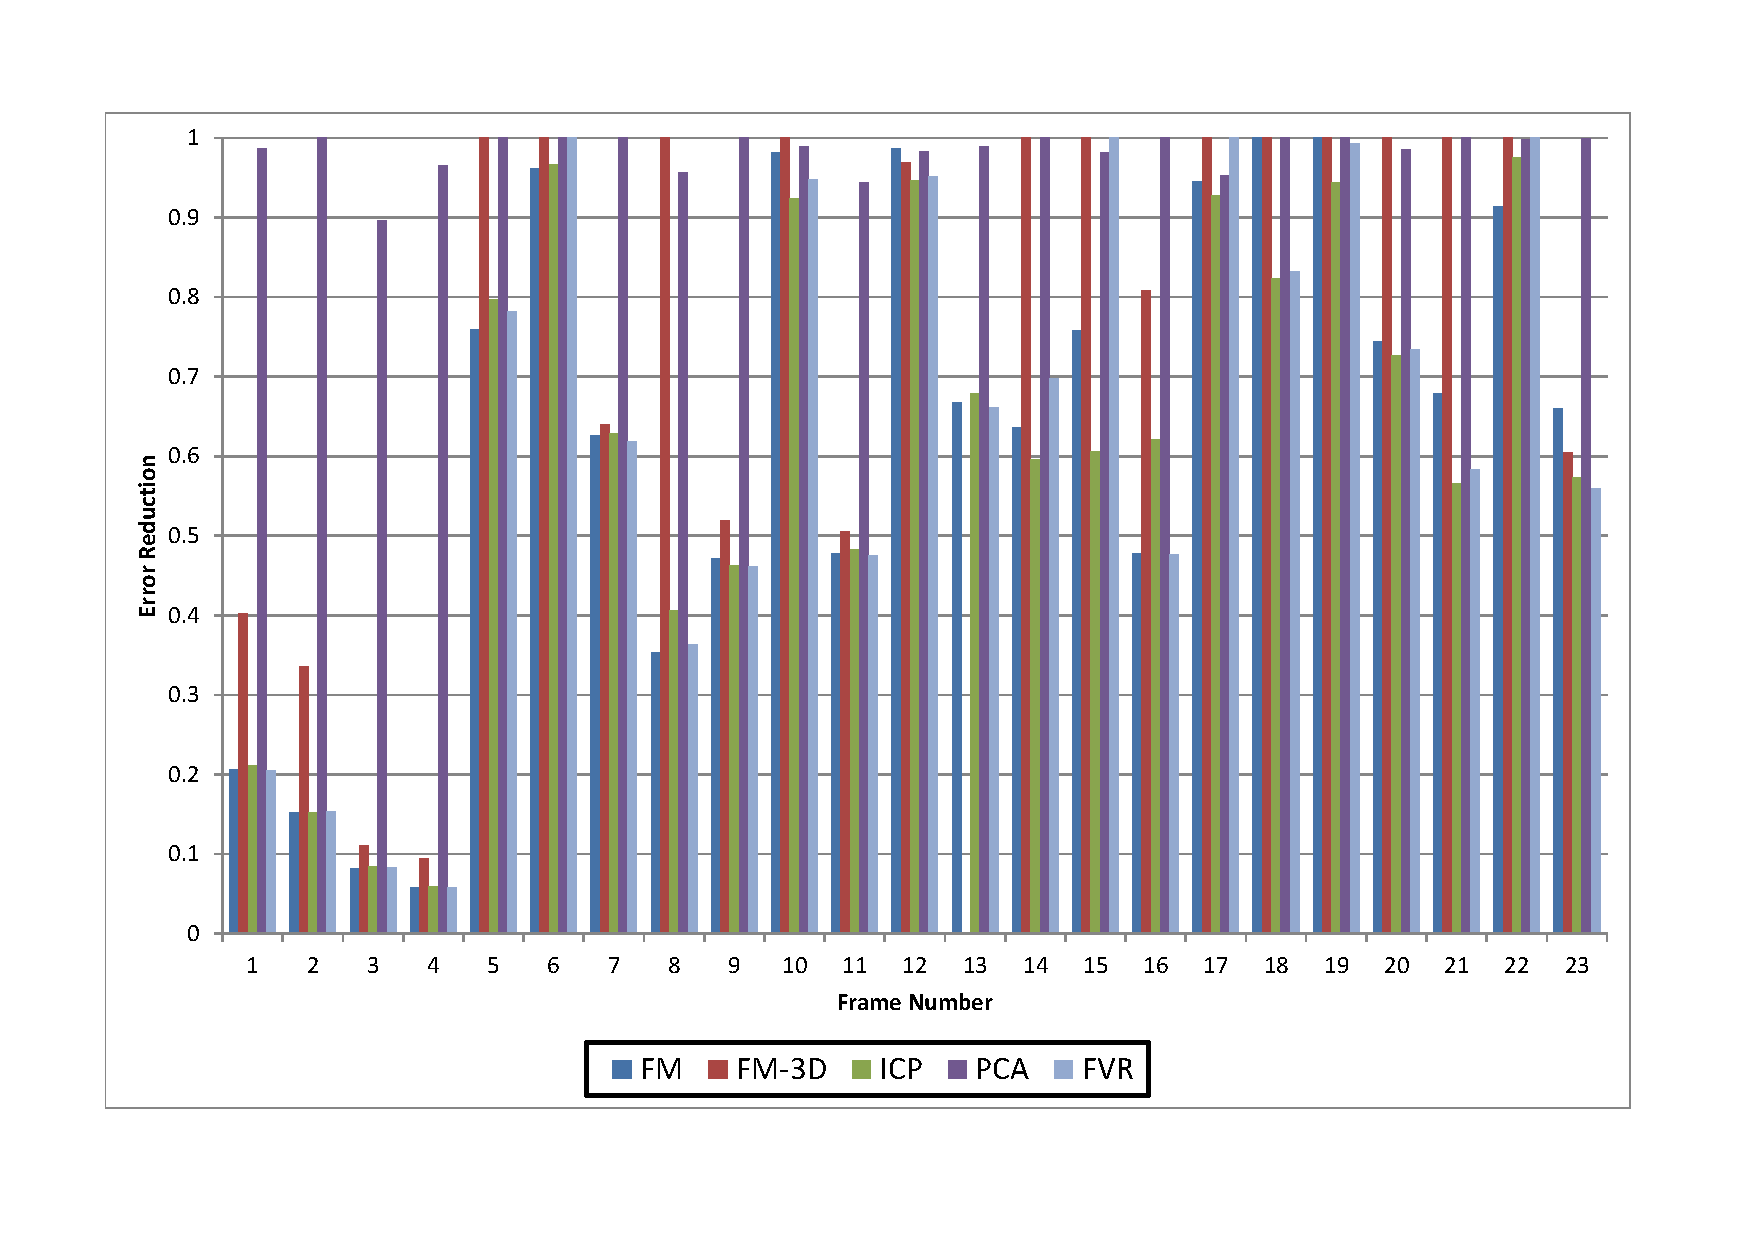
\includegraphics[width=6.0in]{images/results/Office_Texture_Rotation}
\caption{Registration Error for the Office Y-Axis Rotation Data Set}
\label{fig:PET11}
\end{figure*}

Figure \ref{fig:PET11} shows the registration errors for the Office data-set with camera rotation about the Y-axis. Here, in around 50\% of the cases, FVR outperformed or matched the best result. 2D-feature-matching was next best matching or outperforming the best result around 34\% of the time. Interestingly, PCA performed the worst with this data-set. Because rotation can incur a smaller overlap and thus a large shift in the axes and mean of the principal components, this could be expected.

\begin{figure*}[t]
\centering
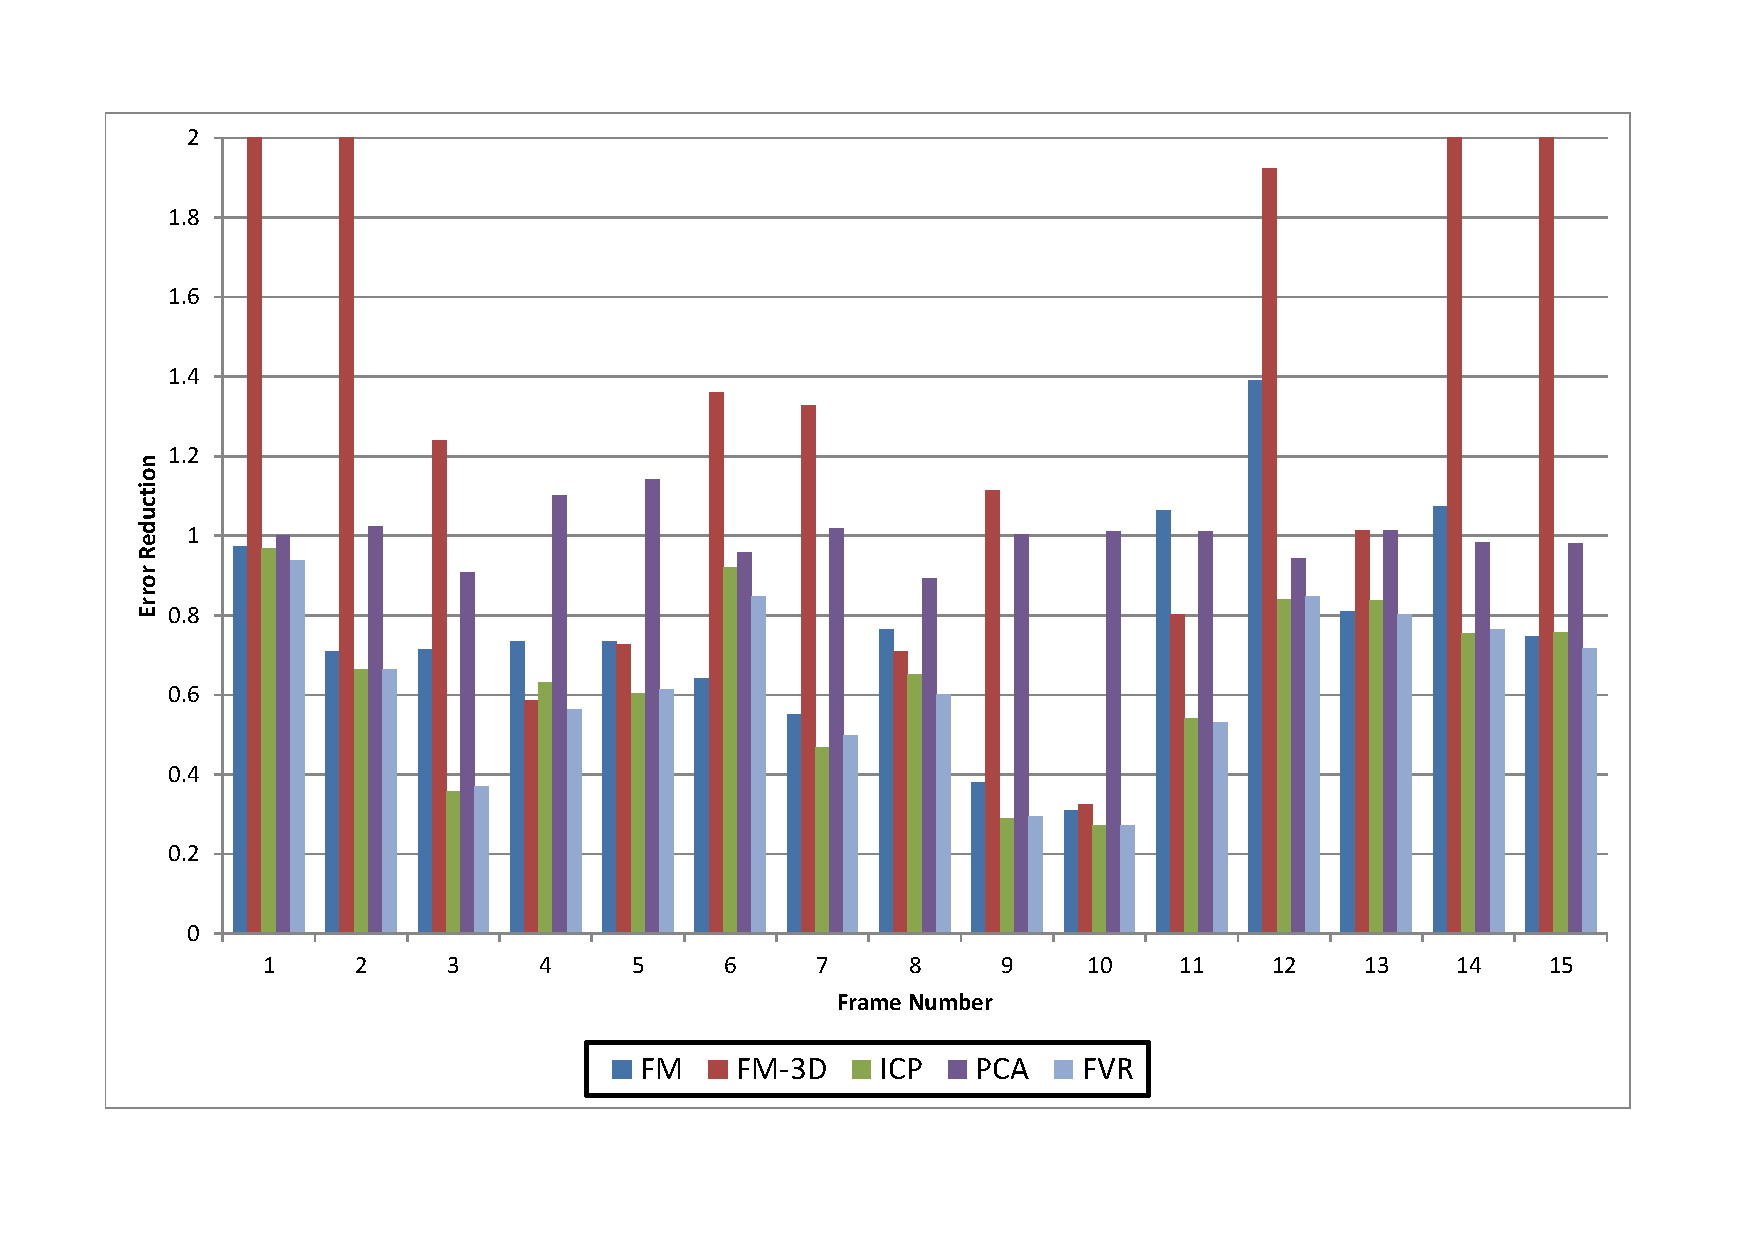
\includegraphics[width=6.0in]{images/results/Office_Texture_Translation}
\caption{Registration Error for the Office Translation Data Set}
\label{fig:PET12}
\end{figure*}

In the Office translation scene, FVR outperformed or matched the other algorithms around 85\% of the time. This shows that the FVR has high accuracy when dealing with translation detection and the registration of 3D data with only translational changes. Here, PCA and 3D-feature matching performed the worst with ICP and 2D-feature matching also being quite consistent and robust.

\begin{figure*}[t]
\centering
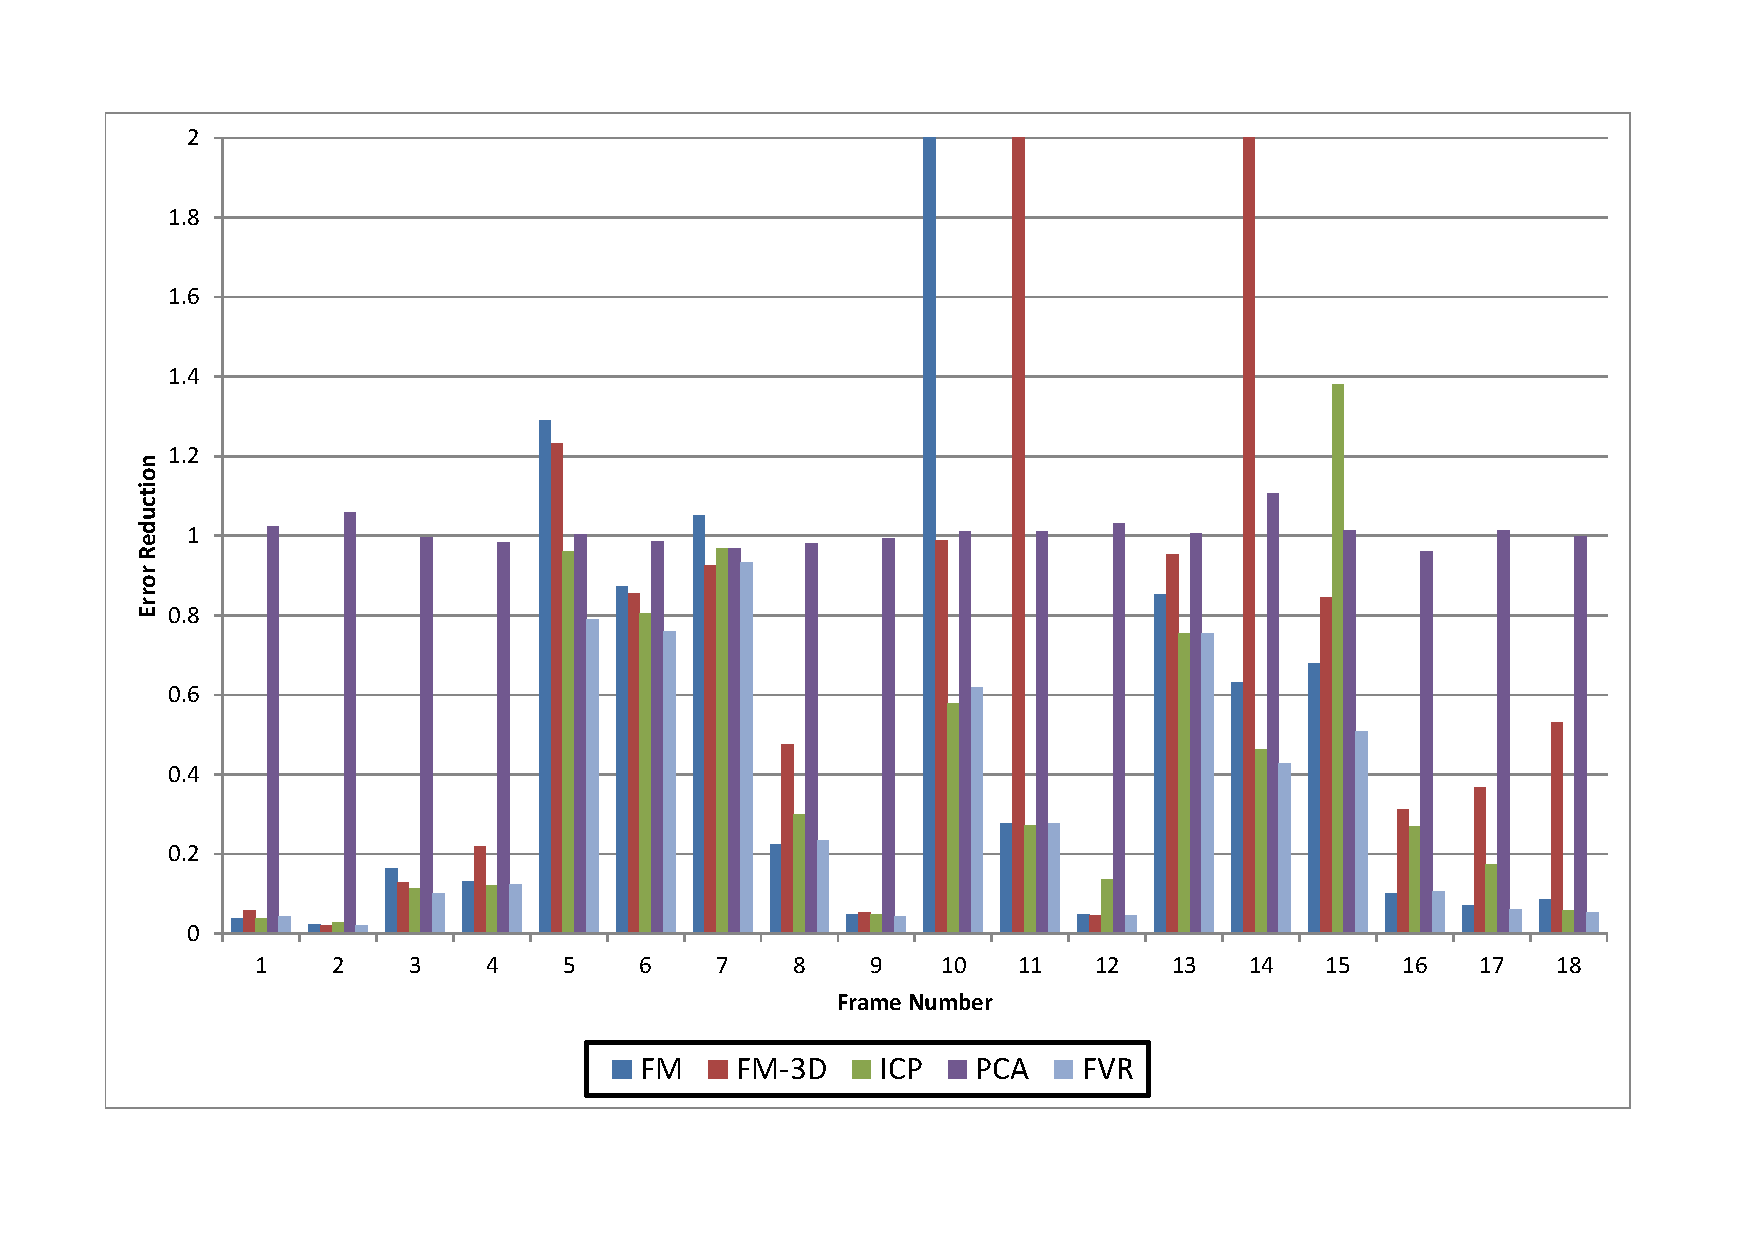
\includegraphics[width=6.0in]{images/results/Outside_No_Texture_Rotation}
\caption{Registration Error for the Little Texture Outdoors Rotation Data Set}
\label{fig:PET13}
\end{figure*}

Figure \ref{fig:PET13} shows results for an outdoors scene with little texture, here the camera was rotated about an origin. In this case, PCA performed the worst, and 3D-feature-matching also failed several times. The only algorithm which did not fail once was FVR. In this test, FVR outperformed or matched the other algorithms 88\% of the time. This can be explained by FVR's robustness to out-door scenes and scenes with little texture. 

\begin{figure*}[t]
\centering
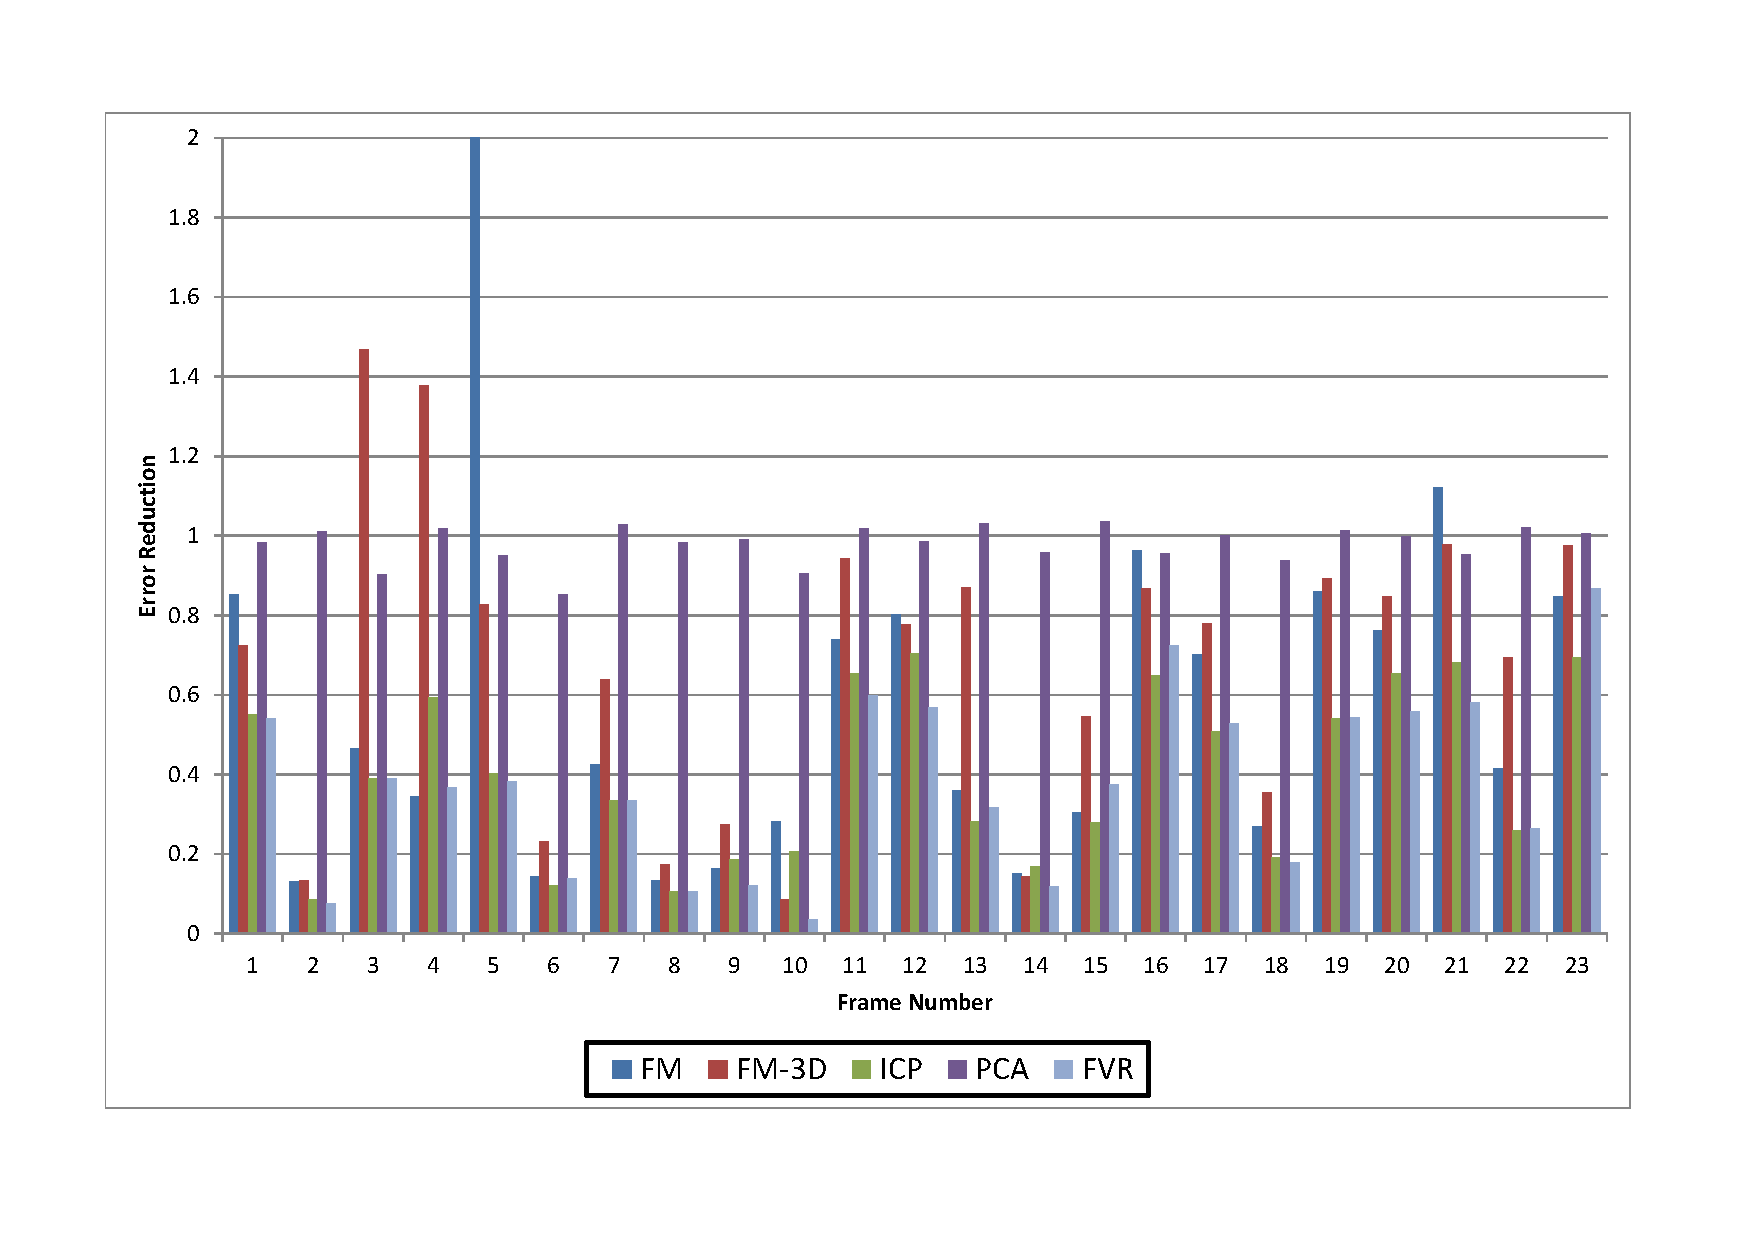
\includegraphics[width=6.0in]{images/results/Outside_No_Texture_Translation}
\caption{Registration Error for the Little Texture Outdoors Translation Data Set}
\label{fig:PET14}
\end{figure*}

Another test using a low-textured out-doors scene was tested where the camera was translated along a path. Results are shown in figure \ref{fig:PET14}. Here again the FVR method dominated recording either the best result or matching best result for around 73\% of the frames. Notably, PCA performed poorly, and both the feature-matching methods failed to register a few times. ICP was more consistent, recoding the best or equivalent result around 47\% of the time. Again, this shows the strength of the FVR method in out-door and low-texture environments. 

\begin{figure*}[t]
\centering
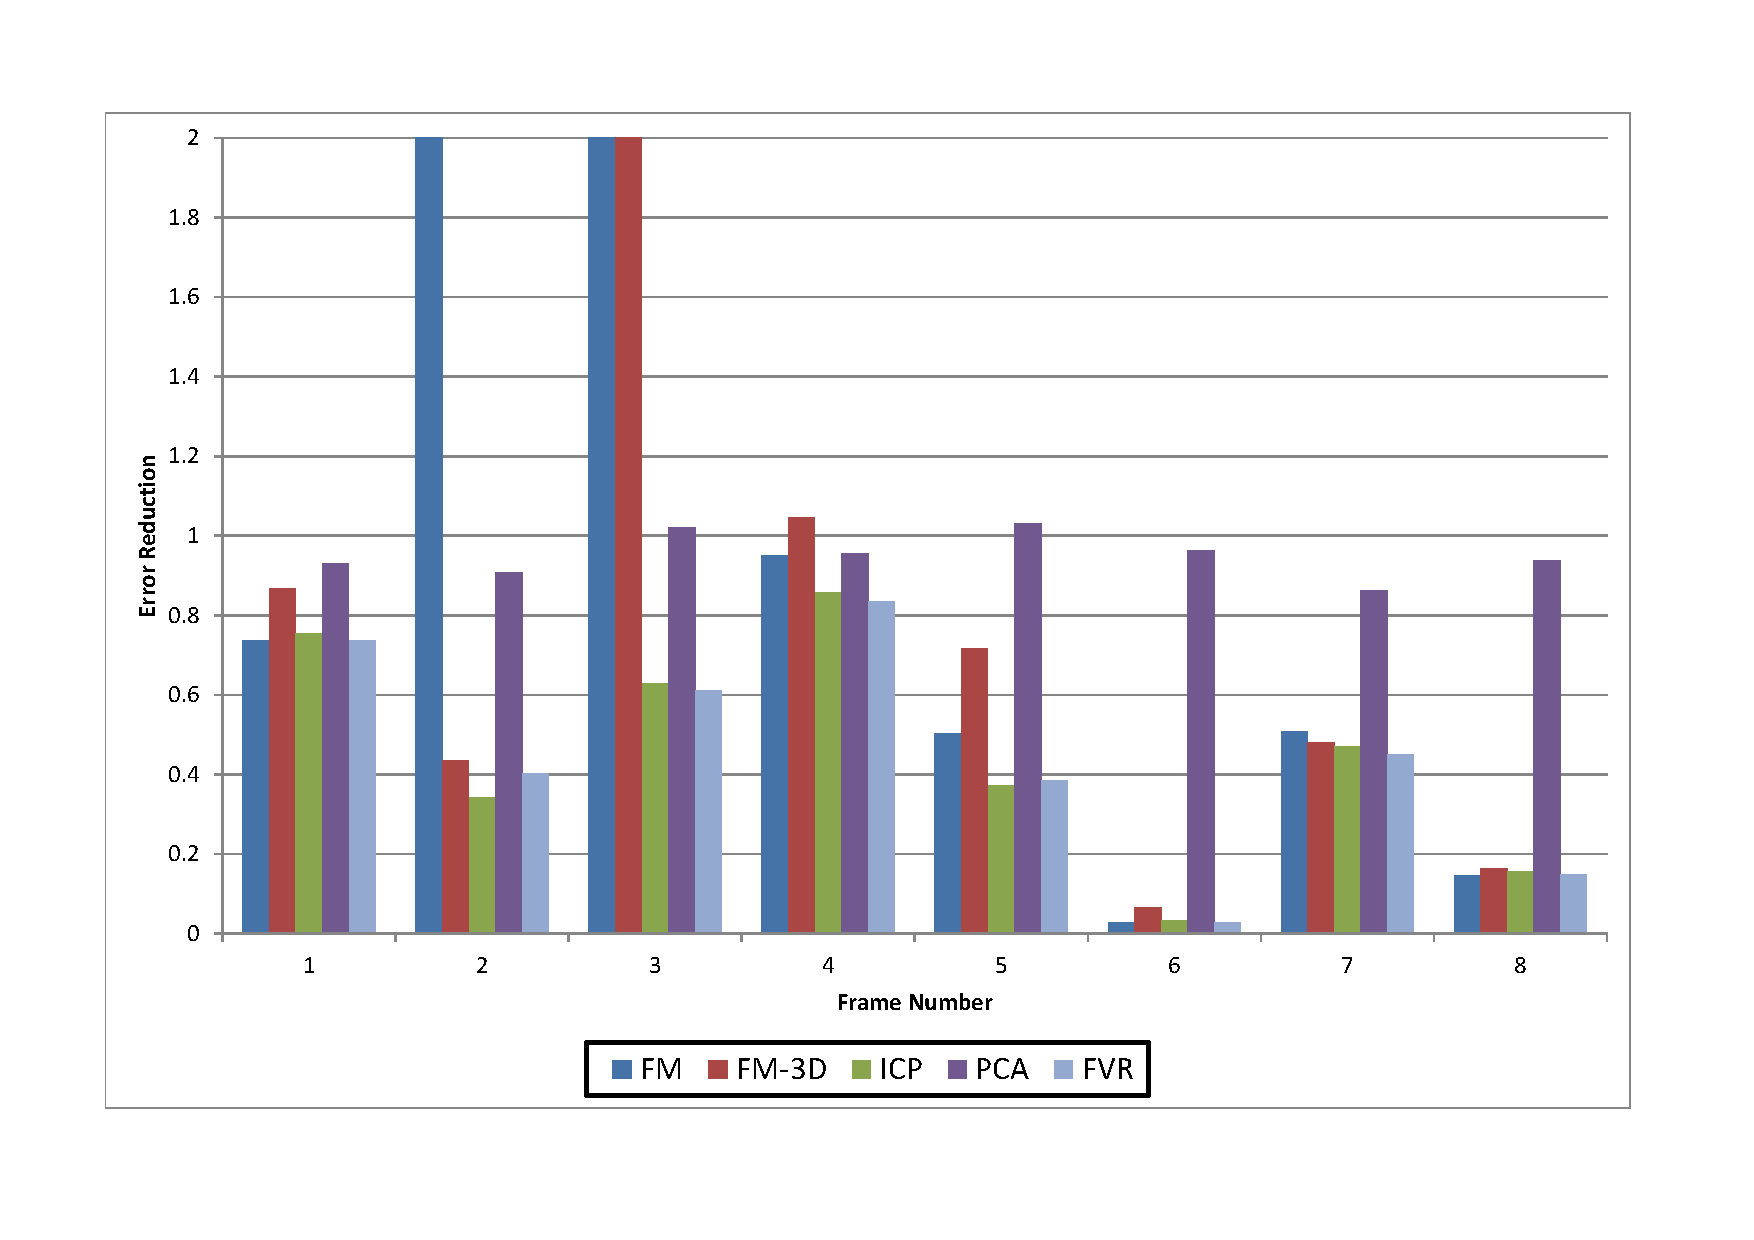
\includegraphics[width=6.0in]{images/results/Outside_TextureConfusion_Rotation}
\caption{Registration Error for the Outdoors Texture Confusion Rotation Data Set}
\label{fig:PET15}
\end{figure*}

Another test was performed with an outdoors scene. Here only 8 of the frames had any good results for all algorithms. They are shown in figure \ref{fig:PET15}. In these results, 6 out of the 8 frames had either a matching or best registration for the FVR method. 2D-feature-matching and 3D-feature-matching both failed a few times, and PCA was inconsistent. ICP had a competitive result 3 out of the 8 times, both FVR and ICP were most consistent. 

\begin{figure*}[t]
\centering
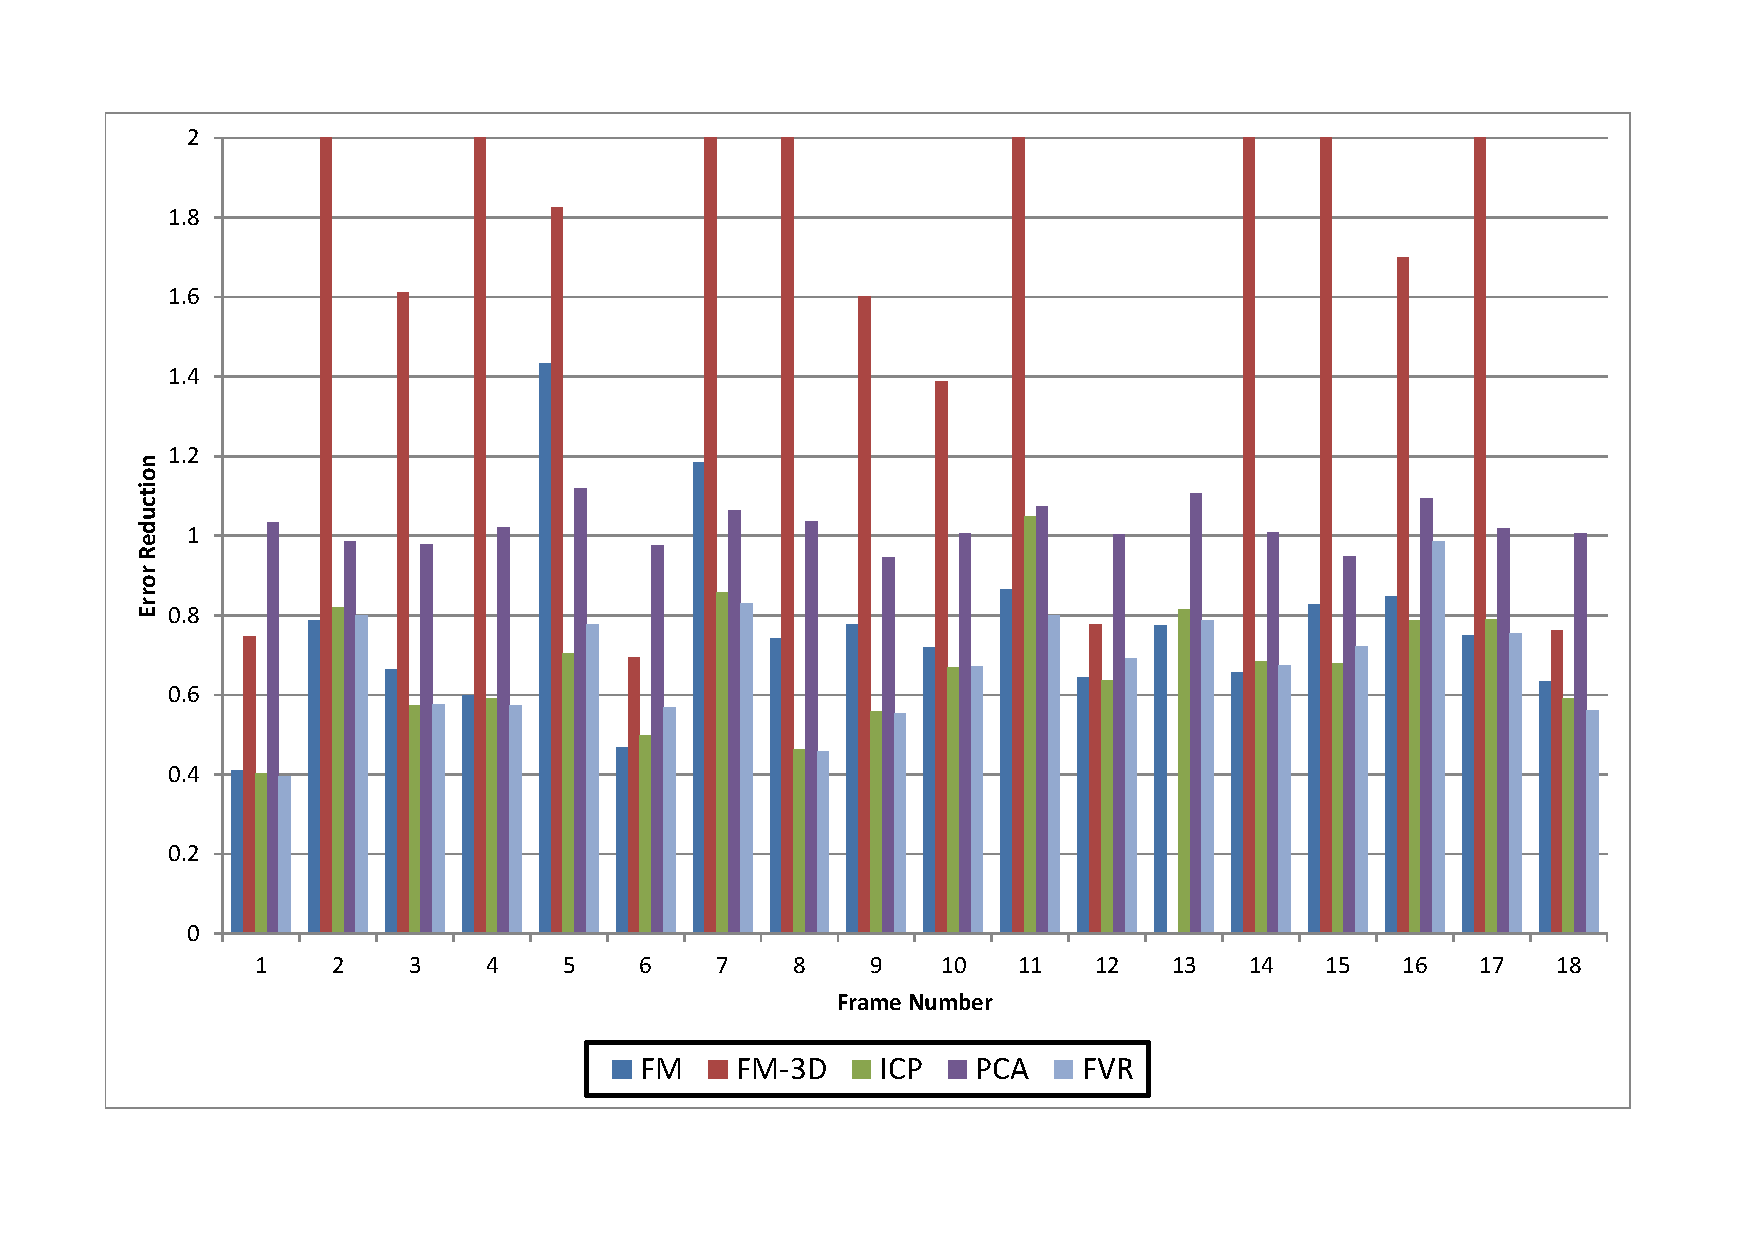
\includegraphics[width=6.0in]{images/results/Outside_TextureConfusion_Translation}
\caption{Registration Error for the Outdoors Texture Confusion Translation Data Set}
\label{fig:PET16}
\end{figure*}

Another scene with texture-confusion was taken out-doors. The interesting results are shown in figure \ref{fig:PET16}. Here, 3D-feature matching failed a majority of the time. Interestingly PCA also failed, the likely reason is because of the amount of noise in an out-doors scene. This noise can give inconsistencies in the principal axes and mean computation. Again, FVR performed best with it getting the best or equivalent result around 55\% of the time. This is another experiment where FVR is shown to be highly robust to scenes with texture confusion. 

\begin{figure*}[t]
\centering
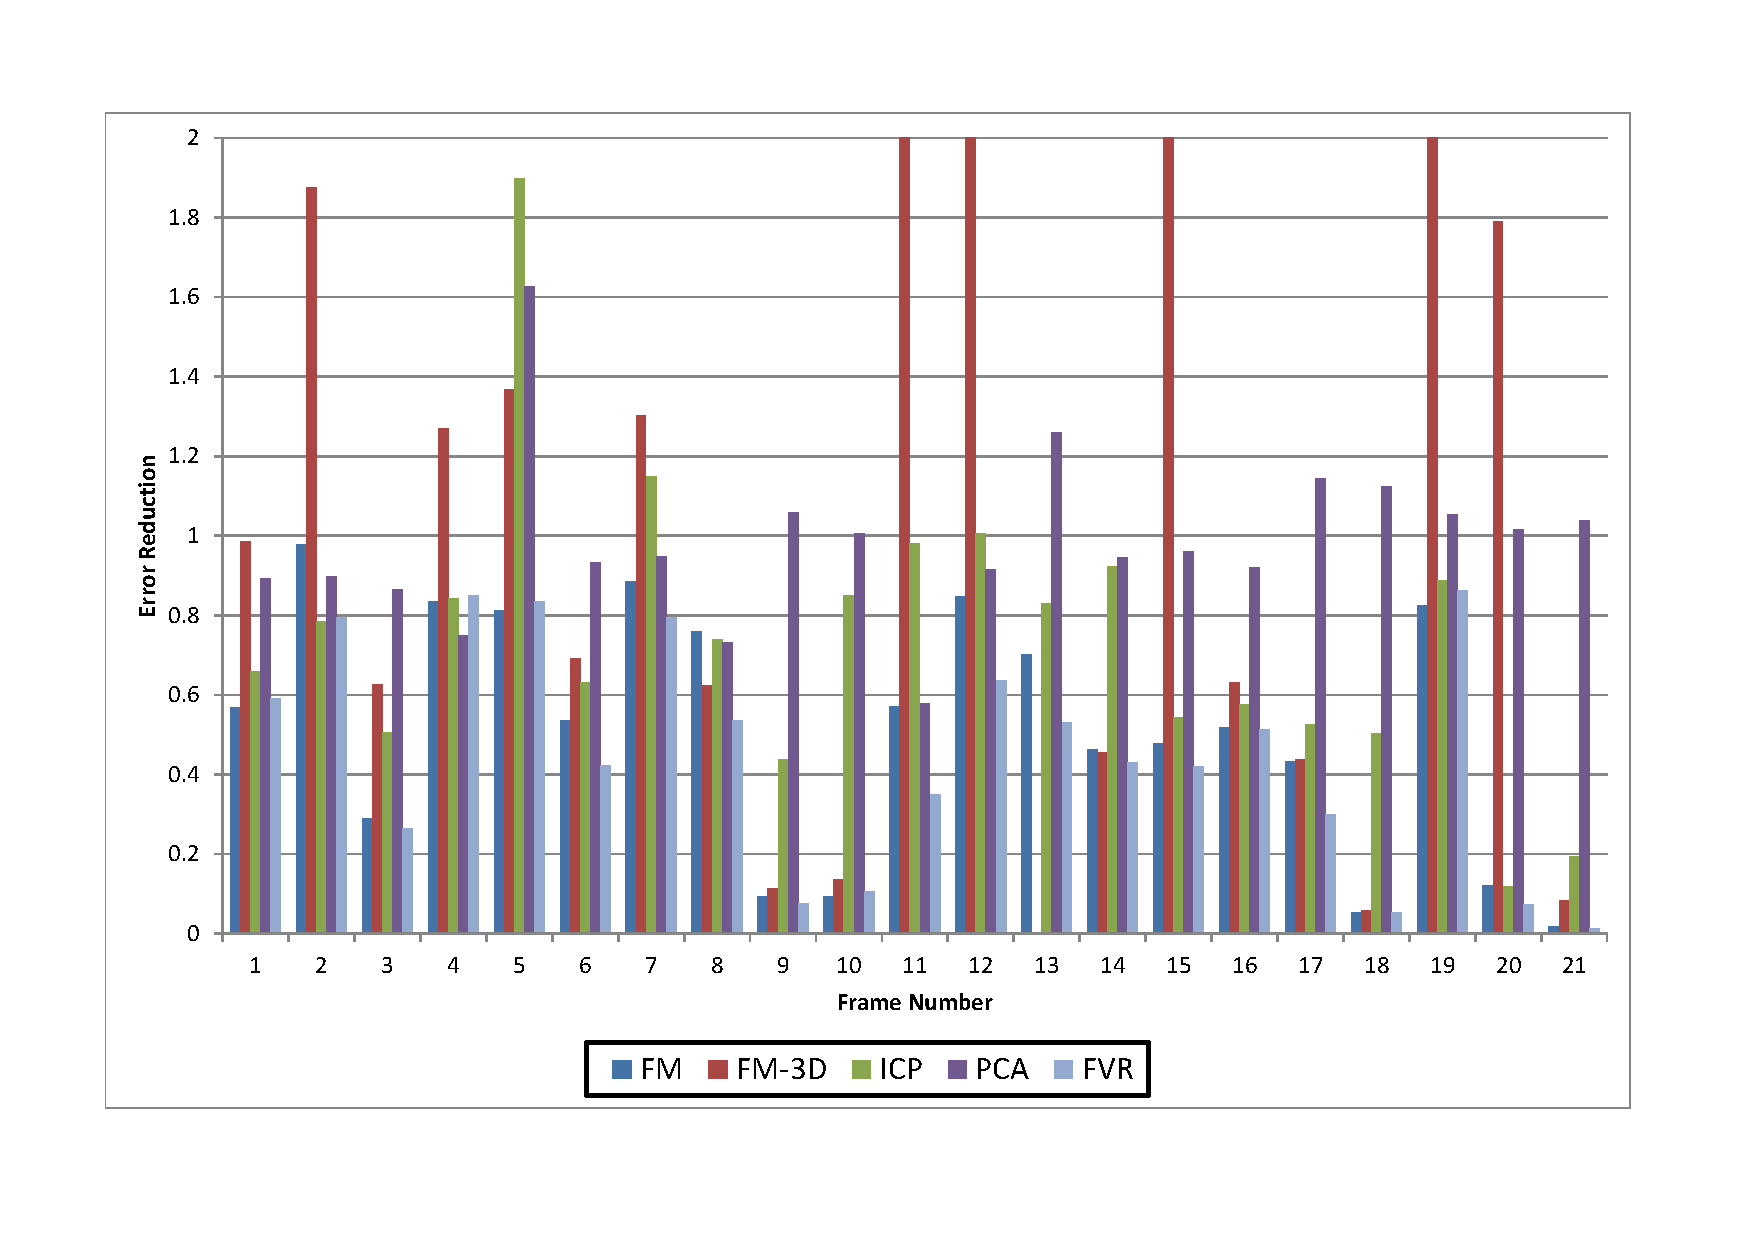
\includegraphics[width=6.0in]{images/results/Plants_Outdoors_Texture_Confusion_Rotation}
\caption{Registration Error for the Outdoor Plants Texture Confusion Rotation Data Set}
\label{fig:PET17}
\end{figure*}

The final figure in the pose estimation tests shows another scene taken out-doors. This scene also contains texture confusion, but the camera was rotated about an axis rather than translated in this data-set. Results shown in figure \ref{fig:PET17} indicate that again FVR dominates with 16 out of the 21 frames having a matching or best registration by FVR. 

\subsection{3D Registration Results}



\subsection{Noise Robustness Results}



\section{Conclusion}
